\clearpage
\section{Result for Savitzky–Golay filter} \label{cap:ResultMODWTRA}

The result presented in this section are denoised with Savitzky–Golay filter and are
 divided into normal bed, section \ref{cap:normalSavitz}, and rocking bed \ref{cap:RockSavitx}. Inside both sections are presented the result for each position for the binary and weighted approach.


%%%%%% NORMAL BED %%%%%%
\subsection{Normal Bed} \label{cap:normalSavitz}

The participant in this phase has to perform a series of jumps before lying on the mattress due to recreating the increase or decrease of the breath rate between the different sleep stages. This phase aims to understand the feasibility of extracting breath rate from the mat. For this phase, the mattress is placed on a standard bed.

%%%%%% NORMAL BED - SUPINE %%%%%%

\subsubsection{Result Normal Bed in Supine Position}  
The estimated respiratory rate per minute (rpm) while the participants are supine with the mattress placed on a normal bed is further presented. Table \ref{tab:SupineNormalStillsg} presented the estimated rpm using binary and weighted approach compared with the rpm given by the ground truth. The approaches retrieve an almost identical rpm, this result may be due to the choice of the minimum confidence value at 80\% that allows keeping only the best signal, maybe with higher confidence can be seen a higher difference between the two approaches. 

\vspace{0.5cm}
\begin{table}[h]
    \centering
    \begin{tabular}{|c|c|c|}
 
    \hline 
    Binary & Weighed & RPM (NOXA1) \\ 
    \hline 
    12.8529  & 12.8333  & 13.485  \\ 
    12.0909  & 12.0909  & 13.1443  \\ 
    11.9167  & 11.9167  & 12.5154  \\ 
    13.3333  & 13.4  & 13.117  \\ 
    12.2857  & 12.2857  & 13.6077 \\ 
    12.5833  & 12.3077  & 13.8993 \\ 
    11.6  & 11.6 & 12.0681  \\ 
    9 &  9  & 11.4768  \\ 
    11.1667  & 10.625  & 12.1549  \\ 
    14.5 & 14.5  & 12.8028 \\ 
    14.3333  & 14.3333  & 12.3275  \\ 
    11.625  & 11.625  & 10.9785  \\ 
    13.125  & 13.125  & 11.8441  \\ 
    13.1111  & 13.1111  & 12.6438  \\ 
    13.3077  & 13.3077  & 11.5351  \\ 
    13.6667  & 13.6667  & 11.99  \\ 
    11.5  & 11.5  & 11.9868 \\ 
    11.4545  & 11.2308  & 11.7824 \\ 
    \hline 
\end{tabular}
\caption{Estimated rpm using binary and weighted approach of the pipeline
compared with the rpm given by the ground truth
- Normal bed and supine position}
\label{tab:SupineNormalStillsg}

\end{table}

Table \ref{tab:SupineNormalStillMetricssg} present the average rpm for both approaches  
and the relative mean absolute error (MAE) and mean absolute percentage error (MAPE). As just discussed in the previous paragraph there is no substantial difference between the two different approaches. The data on which to focus more is the number of breaths that the algorithm misses, represented by MAE and expressed in percentage by MAPE. The average number is 2rpm, which means that if we consider the estimated average of 14.5rpm the error is almost 20\%, quite high for an approach that must be used in the medical field.

%\vspace{0.5cm}
\begin{table}[h]
    \centering
    \begin{tabular}{|c|c|c|}
    \hline 
    & Binary SGf & binary Waveleft & weighed  SGf & weighed Waveleft \\ 
    \hline 
    rpm mean &    \\ 
    MAE resp & 1.0796 &       1.1422  \\ 
    MAPE resp & 8.7793 \%  & 9.2789 \% \\ 
    \hline 
    \end{tabular}
    
    \caption{Evarage number of breath for each approach with the relative mean
    absolute error (MAE) and mean absolute percentage error (MAE) - Normal bed
    and supine position}
    \label{tab:SupineNormalStillMetricssg}    
\end{table}
    
    

Figure \ref{fig:baln1} show the Bland–Altman plot, presented in section \ref{cap:plottino}, of the estimated rpm from the pipeline compared to the value of the ground truth. It helps to visualize the data from Table \ref{tab:SupineNormalStillMetricssg} in respect of the error. Since the result for the approaches is similar the data presented with this plot refers to the weighted approach only.

Figure \ref{fig:rec} shows the denoised signal using MODWTMRA with the highest accuracy (92\%) for the supine position with a normal mattress.

\begin{figure}[p]
  \centering
  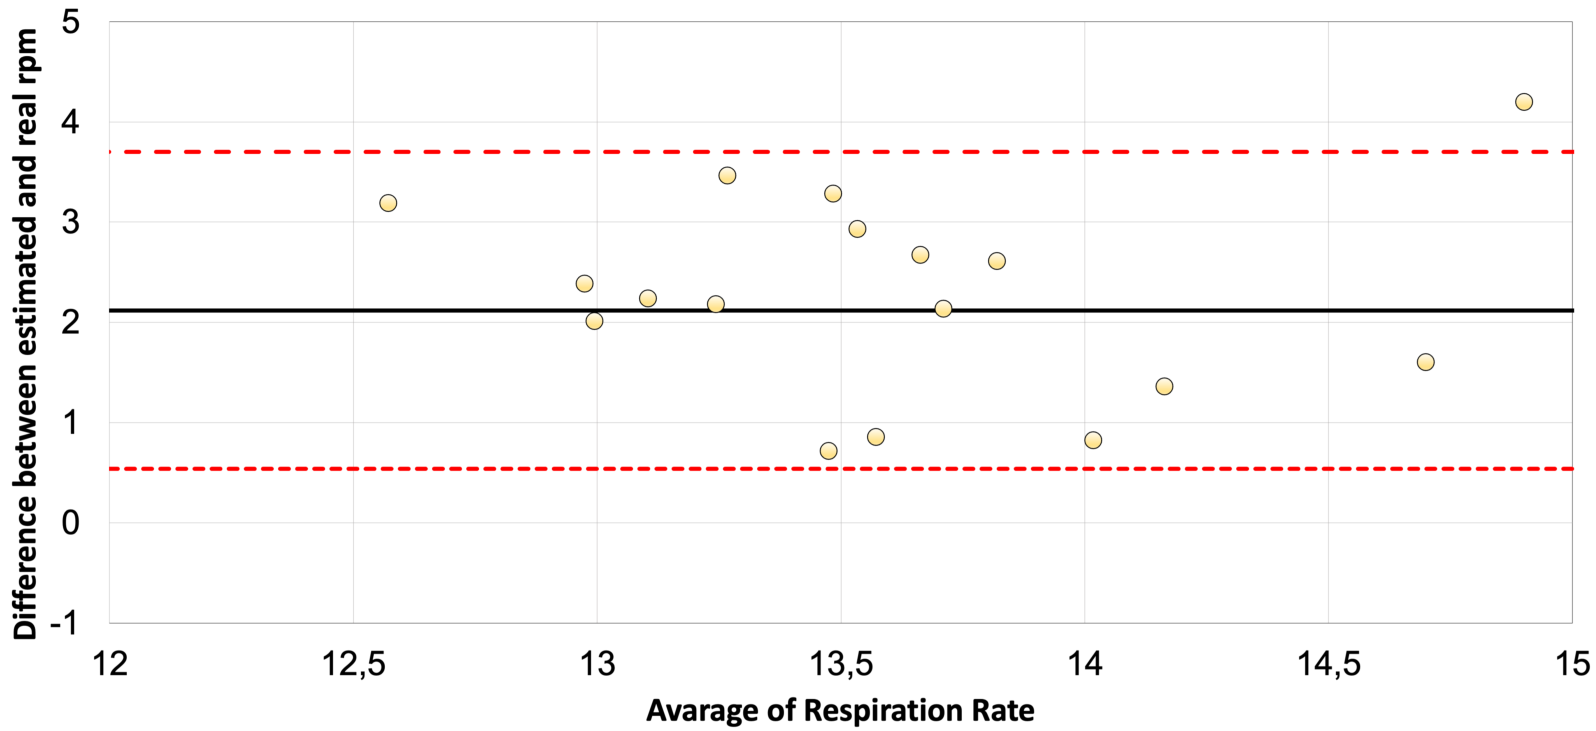
\includegraphics[width=\textwidth]{img/balnd1.pdf}

  \caption{Bland Altman Plot of estimated rpm from the pipeline compared to the value of the ground truth - Normal bed and supine position}
  \label{fig:baln1}
  \vspace{1.5cm}
  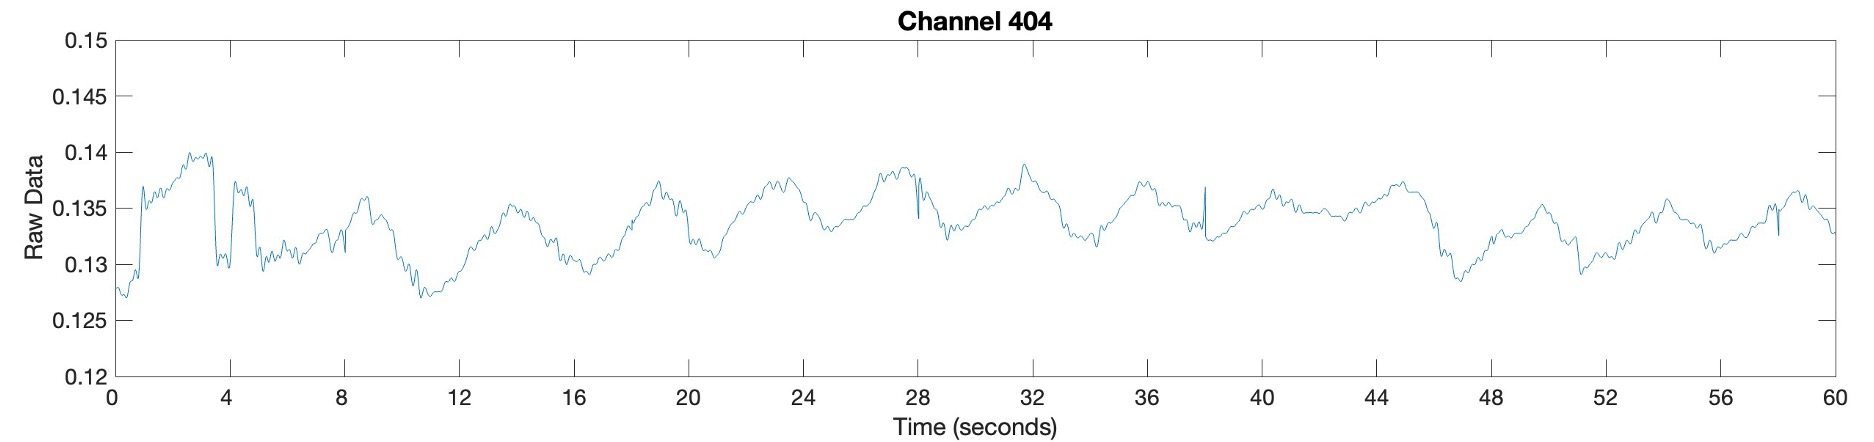
\includegraphics[width=\textwidth]{img/404.jpg}
  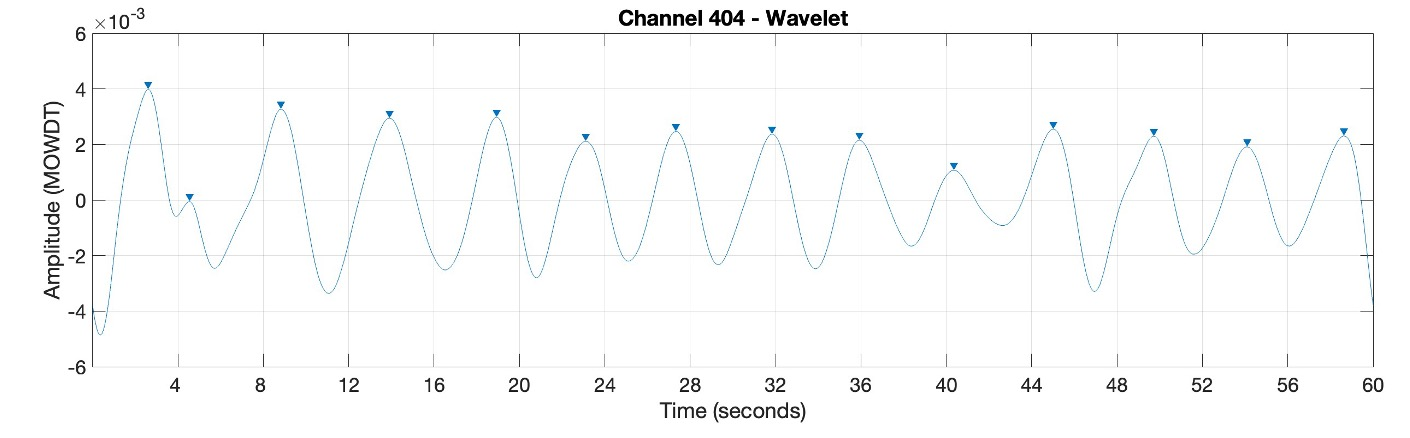
\includegraphics[width=\textwidth]{img/404_wave.jpg}
\caption{Raw data and denoised signal using MODWTMRA of the channel with the highest percentage of confidence (92\%) - Normal bed and supine position}
  \label{fig:rec}
\end{figure}


%%%%%% NORMAL BED - LEFT %%%%%%
\subsubsection{Result Normal Bed in Left Side Position}   \label{cap:ResultNormalBed2}

The estimated respiratory rate per minute (rpm) while the participants are on the left side with the mattress placed on a normal bed is further presented. Table \ref{tab:LeftNormalStill} presented the estimated rpm using binary and weighted approach compared with the rpm given by the ground truth. The approaches retrieve an almost identical rpm, this result may be due to the choice of the minimum confidence value at 80\% that allows keeping only the best signal, maybe with higher confidence can be seen a higher difference between the two approaches. 

\vspace{1.3cm}
%\begin{table}\begin{tabular}{|llllll|}
\hline 
Binary SGf & binary Waveleft & weighed  SGf & weighed Waveleft & resp rate & toolbox \\ 
\hline 
13.375 & 14.6364 & 13.375 & 14.6364 & 11.2045 & 10 \\ 
13.6667 & 15 & 13.6667 & 15 & 12.7397 & 11 \\ 
14 & 16 & 13.5 & 15.25 & 13.0613 & 12 \\ 
14.3571 & 14.2 & 14.3571 & 14.2 & 12.2669 & 12 \\ 
14 & 19 & 14 & 19 & 12.1628 & 13 \\ 
12.8 & 15 & 12.6667 & 14.5 & 13.6039 & 13 \\ 
11.8 & 14.2222 & 11.8 & 14.2222 & 13.1398 & 13 \\ 
14 & 15.6667 & 14 & 15.6667 & 11.5445 & 14 \\ 
13.8333 & 14.7 & 13.8333 & 14.7 & 10.77 & 11 \\ 
13.8889 & 15.8571 & 13.8889 & 15.8571 & 14.2216 & 12 \\ 
13.0833 & 15.5556 & 13.0833 & 15.5556 & 13.1656 & 12 \\ 
14.1111 & 16.5714 & 13.7 & 16.5714 & 12.9764 & 12 \\ 
14.2 & 15 & 14.2 & 15 & 10.9055 & 13 \\ 
13.25 & 15.125 & 13.25 & 15.125 & 13.2294 & 11 \\ 
12.7692 & 15.7143 & 12.2857 & 15.5 & 12.8524 & 11 \\ 
13.9167 & 15.2 & 13.6154 & 15.2 & 11.3824 & 13 \\ 
13 & 14.6 & 13 & 14.6 & 13.5579 & 11 \\ 
13 & 15.8889 & 13 & 15.8889 & 11.6069 & 12 \\ 
\hline 
\end{tabular}
\caption{Breath per minutes for each approach, result from Noxtural and toolbox
- Left position still mattress}
\end{table}

\begin{table}[h]
    \centering
    \begin{tabular}{|c|c|c|}
 
    \hline 
    Binary & Weighed &RPM (NOXA1) \\ 
    \hline 
   14.6364  & 14.6364 & 11.2045 \\ 
      15  & 15 & 12.7397 \\ 
      16  & 15.25 & 13.0613 \\  
  14.2  & 14.2 & 12.2669 \\ 
      19  & 19 & 12.1628 \\ 
      15  & 14.5 & 13.6039 \\ 
     14.2222  & 14.2222 & 13.1398 \\ 
     15.6667 & 15.6667 & 11.5445 \\ 
+ 14.7 & 14.7 & 10.77  \\ 
     15.8571  & 15.8571 & 14.2216 \\ 
 15.5556 & 15.5556 & 13.1656\\ 
 16.5714 & 16.5714 & 12.9764 \\ 
   15 &  15 & 10.9055 \\ 
15.125 & 15.125 & 13.2294 \\ 
15.7143& 15.5 & 12.8524 \\ 
     15.2 & 15.2 & 11.3824 \\ 
14.6 &  14.6 & 13.5579 \\ 
15.8889 & 15.8889 & 11.6069 \\ 
    \hline 
    \end{tabular}
    \caption{Estimated rpm using binary and weighted approach of the pipeline
    compared with the rpm given by the ground truth -
    - Normal bed and left side}
    \label{tab:LeftNormalStill}

\end{table}
    

\vspace{0.5cm}

Table \ref{tab:LeftNormalStillMetrics} present the average rpm for both approaches  
and the relative mean absolute error (MAE) and mean absolute percentage error (MAPE). As just discussed in the previous paragraph there is no substantial difference between the two different approaches. The data on which to focus more is the number of breaths that the algorithm misses, represented by MAE and expressed in percentage by MAPE. The average number is 2.5rpm, which means that if we consider the estimated average of 15.3rpm the error is over 24\%, worst than in the supine position, probably due to the smaller contact area between the body and the mattress.

\vspace{1cm}
\begin{table}[H]
    \centering

    \begin{tabular}{|c|c|c|}
    \hline 
    & Binary  & Weighed \\ 
    
    \hline 
    rpm mean & 15.441 & 15.360\\
    MAE resp  &   2.4545 &  2.8934 \\ 
    MAPE  & 24.62\% & 24.0041\% \\ 
    \hline 

    \end{tabular}
    \caption{varage number of breath for each approach with the relative mean
    absolute error (MAE) and mean absolute percentage error (MAE) - Normal bed
    and left side}
    \label{tab:LeftNormalStillMetrics}

    \end{table}
    
\vspace{0.5cm}

Figure \ref{fig:baln2} show the Bland–Altman plot, presented in section \ref{cap:plottino}, of the estimated rpm from the pipeline compared to the value of the ground truth. It helps to visualize the data from Table \ref{tab:LeftNormalStillMetrics} in respect of the error. Since the result for the approaches is similar the data presented with this plot refers to the weighted approach only.

Figure \ref{fig:rec} shows the denoised signal using MODWTMRA with the highest accuracy (92\%) for the supine position with a normal mattress.

\begin{figure}[p]
  \centering
  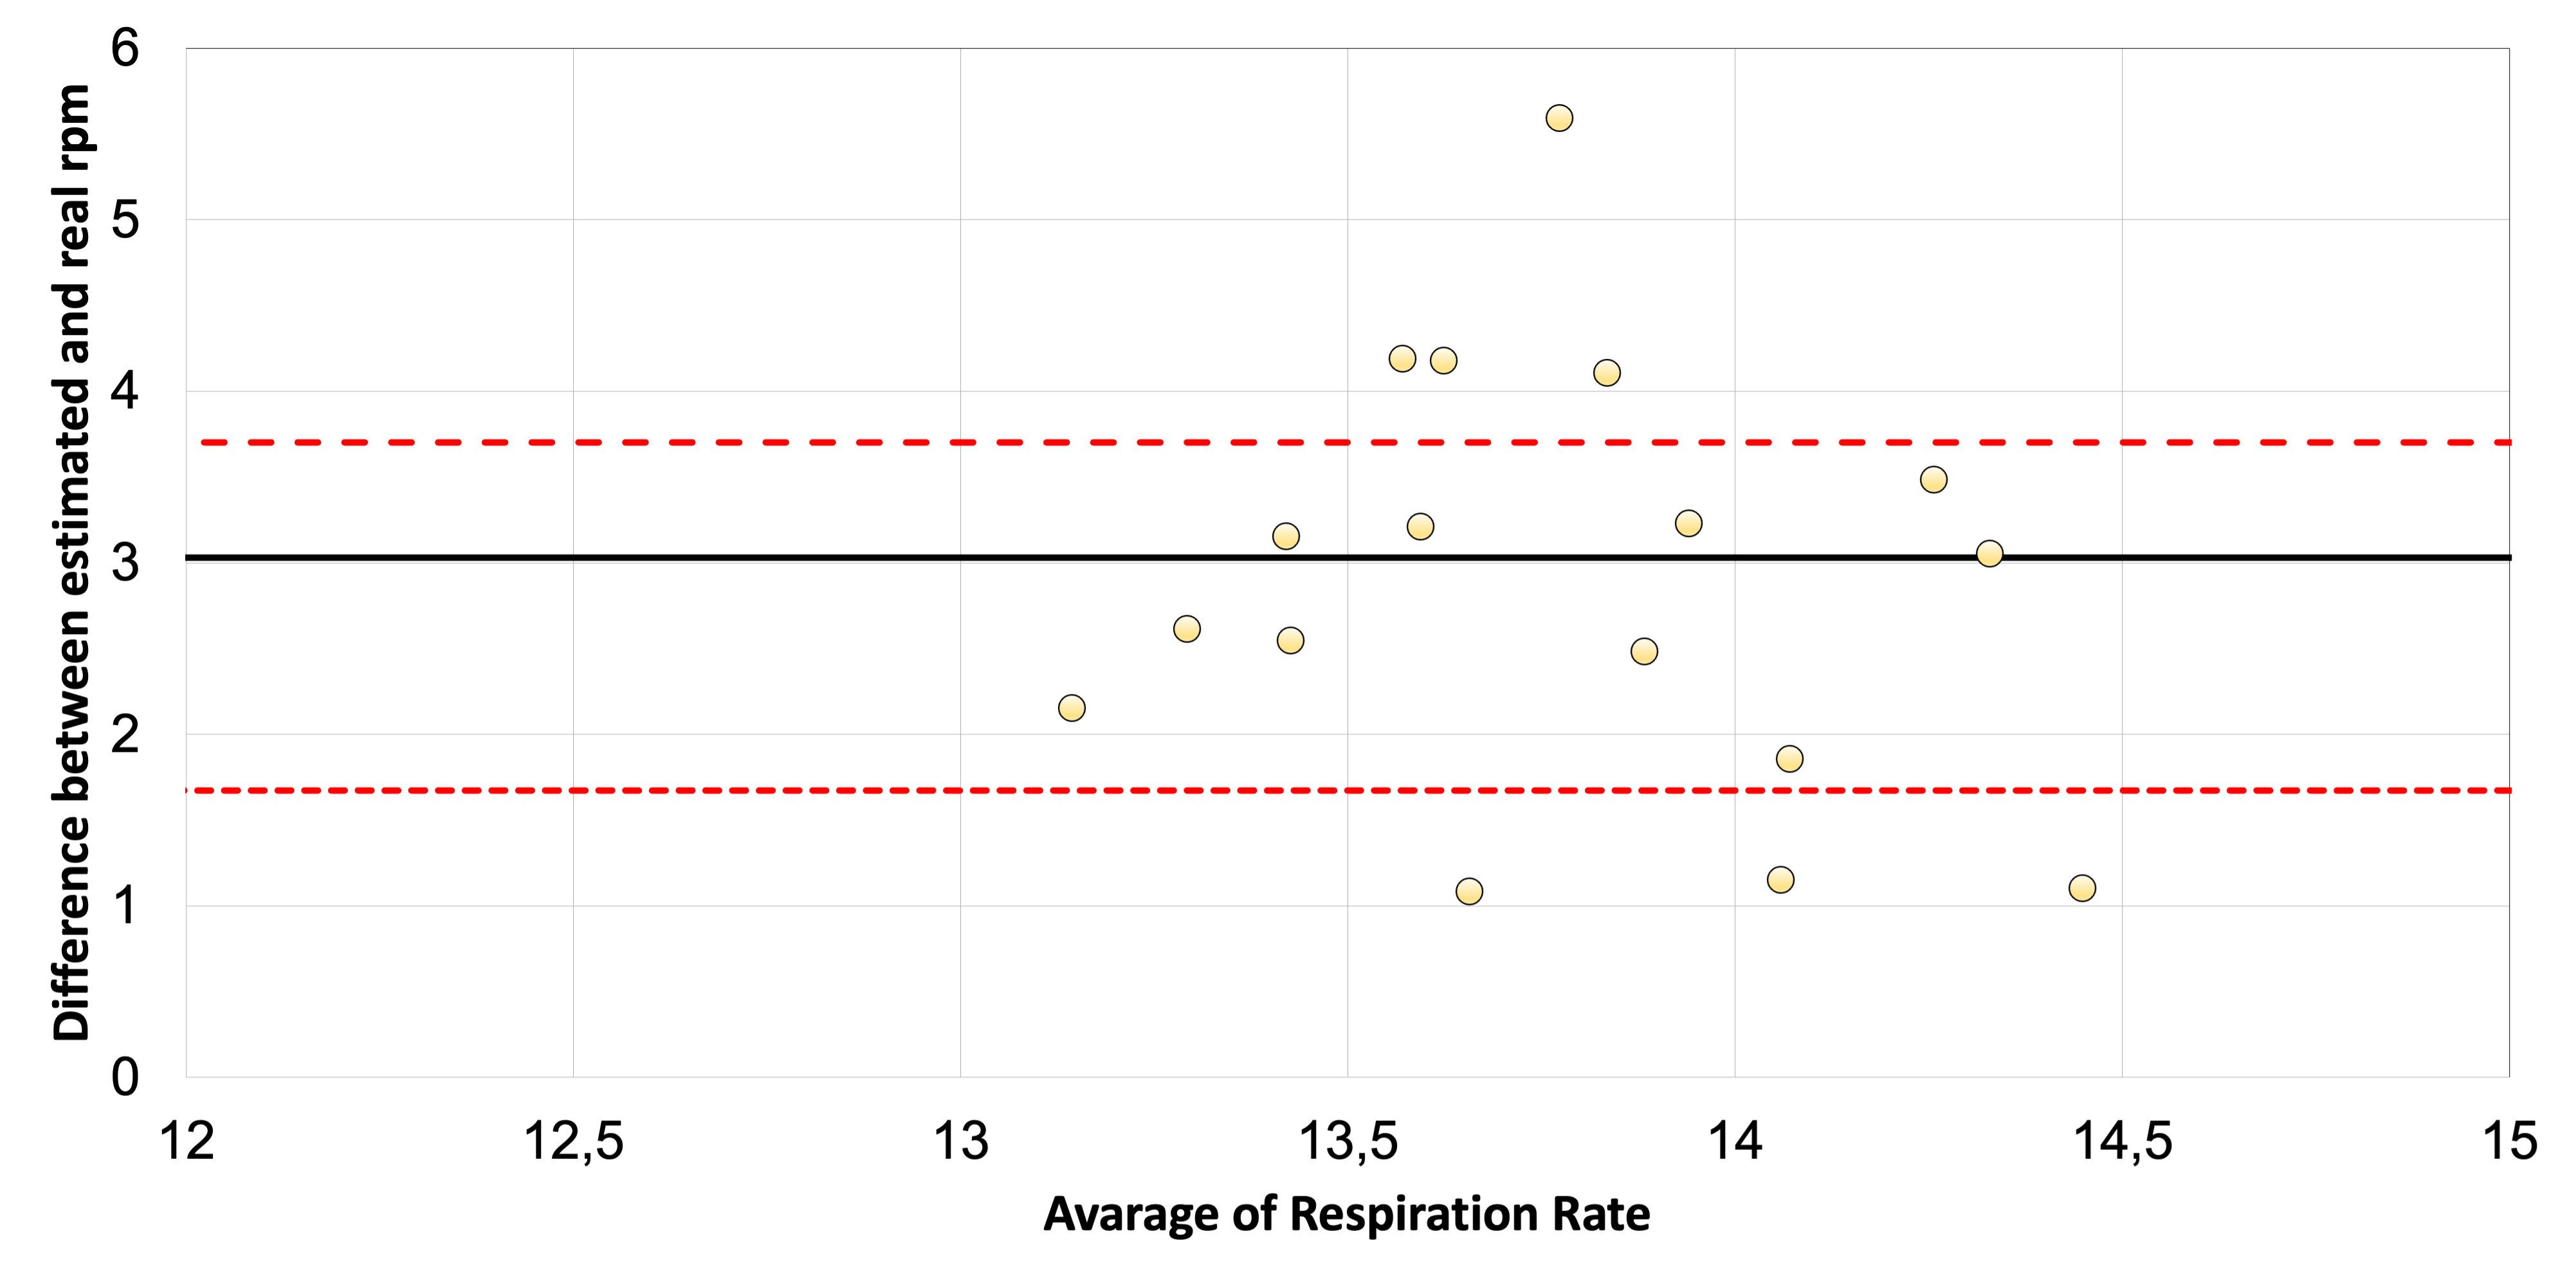
\includegraphics[width=\textwidth]{img/balnd2.png}

  \caption{Bland Altman Plot of estimated rpm from the pipeline compared to the value of the ground truth - Normal bed and left side}
  \label{fig:baln2}
  \vspace{1.5cm}
  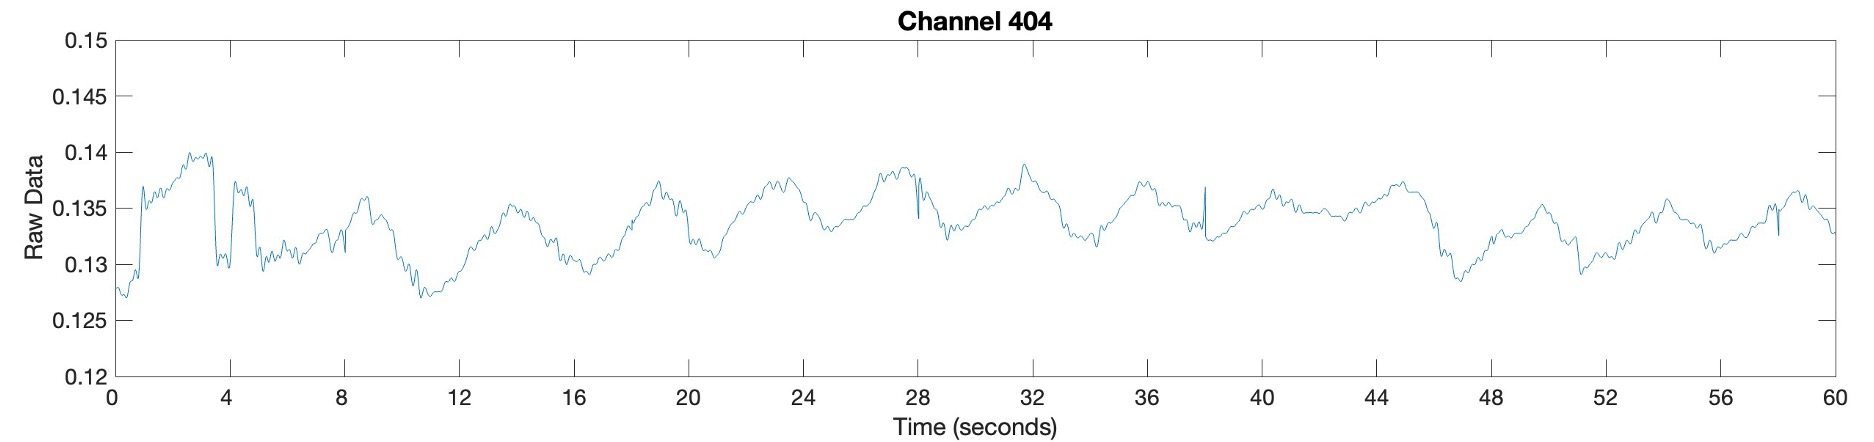
\includegraphics[width=\textwidth]{img/404.jpg}
  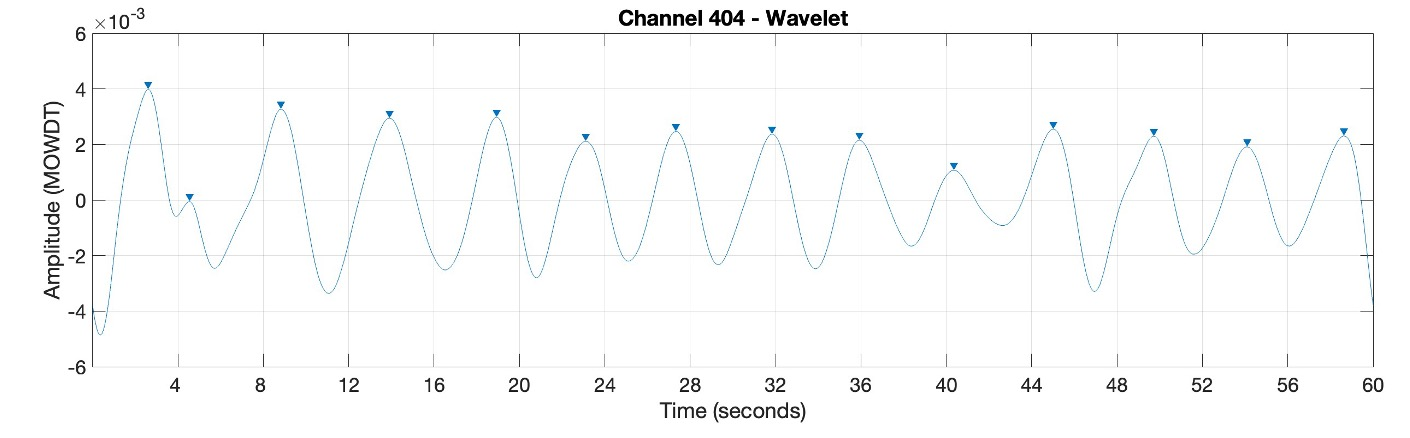
\includegraphics[width=\textwidth]{img/404_wave.jpg}
\caption{Raw data and denoised signal using MODWTMRA of the channel with the highest percentage of confidence (92\%) - Normal bed and supine position}
  \label{fig:rec}
\end{figure}


\clearpage
%%%%%% NORMAL BED - PRONE %%%%%%
\subsubsection{Result Normal Bed in Prone Side Position}   \label{cap:ResultNormalBed3}

The estimated respiratory rate per minute (rpm) while the participants are in the prone position with the mattress placed on a normal bed is further presented. Table \ref{tag:ProneNormalStill} presented the estimated rpm using binary and weighted approach compared with the rpm given by the ground truth. The approaches retrieve an almost identical rpm, this result may be due to the choice of the minimum confidence value at 80\% that allows keeping only the best signal, maybe with higher confidence can be seen a higher difference between the two approaches. 

\vspace{1.3cm}
%\begin{table}\begin{tabular}{|llllll|}
\hline 
Binary SGf & binary Waveleft & weighed  SGf & weighed Waveleft & resp rate & toolbox \\ 
\hline 
13.375 & 14.6364 & 13.375 & 14.6364 & 11.2045 & 10 \\ 
13.6667 & 15 & 13.6667 & 15 & 12.7397 & 11 \\ 
14 & 16 & 13.5 & 15.25 & 13.0613 & 12 \\ 
14.3571 & 14.2 & 14.3571 & 14.2 & 12.2669 & 12 \\ 
14 & 19 & 14 & 19 & 12.1628 & 13 \\ 
12.8 & 15 & 12.6667 & 14.5 & 13.6039 & 13 \\ 
11.8 & 14.2222 & 11.8 & 14.2222 & 13.1398 & 13 \\ 
14 & 15.6667 & 14 & 15.6667 & 11.5445 & 14 \\ 
13.8333 & 14.7 & 13.8333 & 14.7 & 10.77 & 11 \\ 
13.8889 & 15.8571 & 13.8889 & 15.8571 & 14.2216 & 12 \\ 
13.0833 & 15.5556 & 13.0833 & 15.5556 & 13.1656 & 12 \\ 
14.1111 & 16.5714 & 13.7 & 16.5714 & 12.9764 & 12 \\ 
14.2 & 15 & 14.2 & 15 & 10.9055 & 13 \\ 
13.25 & 15.125 & 13.25 & 15.125 & 13.2294 & 11 \\ 
12.7692 & 15.7143 & 12.2857 & 15.5 & 12.8524 & 11 \\ 
13.9167 & 15.2 & 13.6154 & 15.2 & 11.3824 & 13 \\ 
13 & 14.6 & 13 & 14.6 & 13.5579 & 11 \\ 
13 & 15.8889 & 13 & 15.8889 & 11.6069 & 12 \\ 
\hline 
\end{tabular}
\caption{Breath per minutes for each approach, result from Noxtural and toolbox
- Left position still mattress}
\end{table}

\begin{table}[h]
    \centering
    \begin{tabular}{|c|c|c|}
    \hline 
    Binary & Weighed  SGf & RPM (NOXA1) \\ 
    \hline 
     15.7 & 15.7 & 11.5949 \\ 
    15.7333  & 15.7333 & 11.1628\\ 
   16.1  & 16.1 & 11.0005 \\ 
     15.6667 & 15.6667 & 10.4762  \\ 
  15.25  & 15.25 & 10.4723 \\ 
     14.5714 & 14.5714 & 9.5345  \\ 
     15.5714  & 15.5714 & 9.5467 \\ 
    15.875& 15.875 & 13.5758  \\ 
 14  & 14 & 11.1779  \\ 
     14.375  & 14.375 & 9.5345  \\ 
      14.4667  & 14.4667 & 9.5841 \\ 
 14.5  & 14.5 & 11.8196  \\ 
 14.2143 & 14.2143 & 11.8153  \\ 
 13.9474  & 13.9474 & 9.5223  \\ 
   15.037  & 15.037 & 10.8508  \\ 
 14.931  & 14.931 & 10.8876  \\ 
     15.25  & 15.25 & 10.9705  \\ 
     15.3333 & 15.3333 & 11.237  \\ 
    \hline 
    \end{tabular}
    
    \caption{Estimated rpm using binary and weighted approach of the pipeline
    compared with the rpm given by the ground truth - Normal bed and supine position}
    \label{tag:ProneNormalStill}
    \end{table}
    
    

\vspace{0.5cm}

Table \ref{tab:ProneNormalStillMetrics} present the average rpm for both approaches  
and the relative mean absolute error (MAE) and mean absolute percentage error (MAPE). As just discussed in the previous paragraph there is no substantial difference between the two different approaches. The data on which to focus more is the number of breaths that the algorithm misses, represented by MAE and expressed in percentage by MAPE. The average number is 2.8rpm, which means that if we consider the estimated average of 15rpm the error is over 36\%, worst worse than the two previous results it may depend on the movement of the chest in the prone position changes.


\vspace{1cm}
\begin{table}[H]
    \centering
    \begin{tabular}{|c|c|c|}
    \hline 
    & Binary & Weighed \\ 
    
    \hline 

    rpm mean   &  15.029 &  15.029 \\
    MAE rpm & 2.8957 \% &  2.8957\% \\
    MAPE tool  & 36.5982 & 36.5982 \\ 
    \hline 
    \end{tabular}
    
    \caption{Metrics to evaluate the participant in belly position with moving mattress}
    \label{tab:ProneNormalStillMetrics}
    \end{table}
    
\vspace{0.5cm}

Figure \ref{fig:baln2} show the Bland–Altman plot, presented in section \ref{cap:plottino}, of the estimated rpm from the pipeline compared to the value of the ground truth. It helps to visualize the data from Table \ref{tab:ProneNormalStillMetrics} in respect of the error. Since the result for the approaches is similar the data presented with this plot refers to the weighted approach only.

Figure \ref{fig:rec} shows the denoised signal using MODWTMRA with the highest accuracy (92\%) for the supine position with a normal mattress.

\begin{figure}[p]
  \centering
  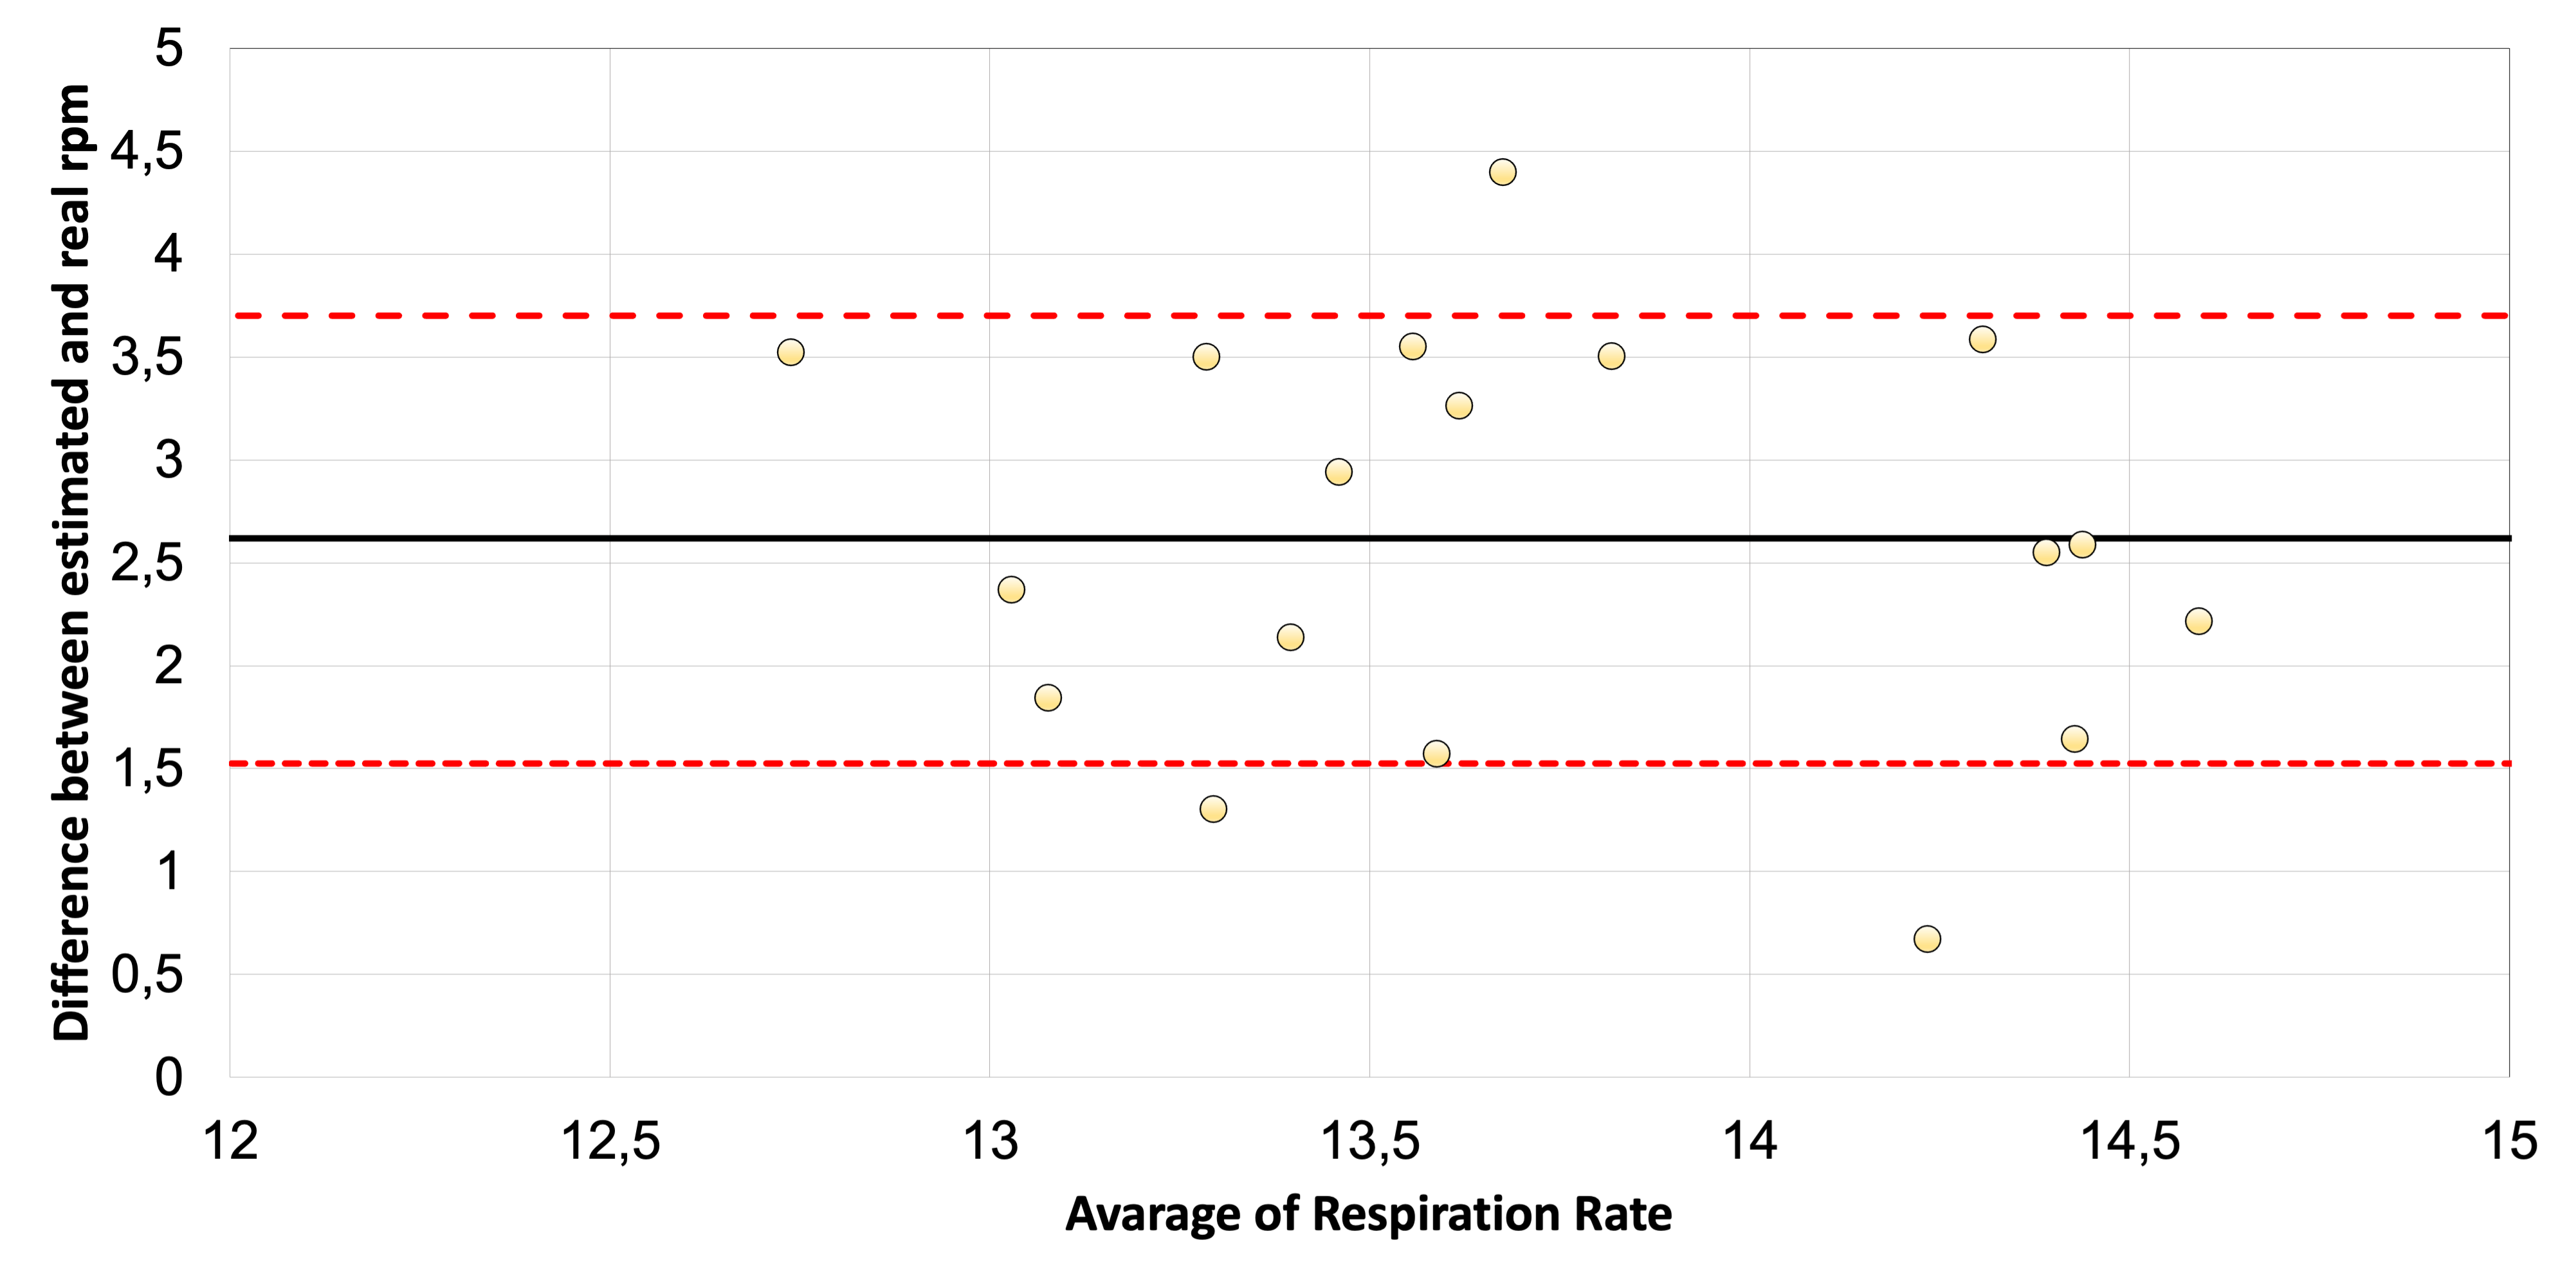
\includegraphics[width=\textwidth]{img/balnd3.png}

  \caption{Bland Altman Plot of estimated rpm from the pipeline compared to the value of the ground truth - Normal bed and prone position}
  \label{fig:baln2}
  \vspace{1.5cm}
  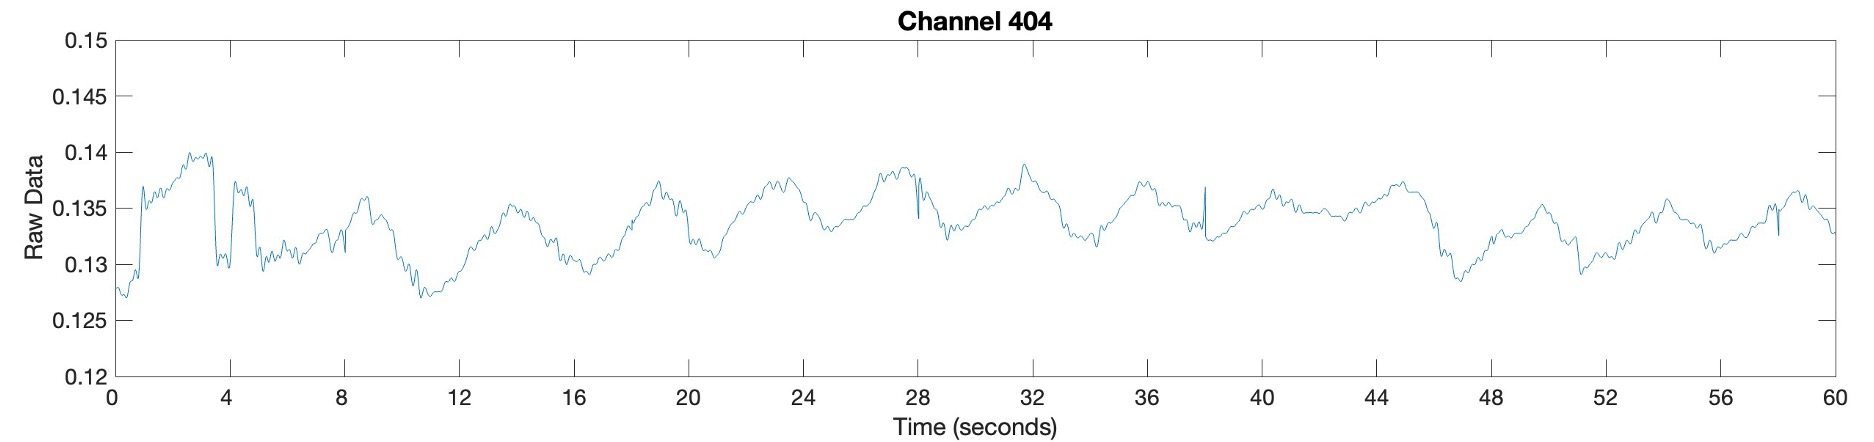
\includegraphics[width=\textwidth]{img/404.jpg}
  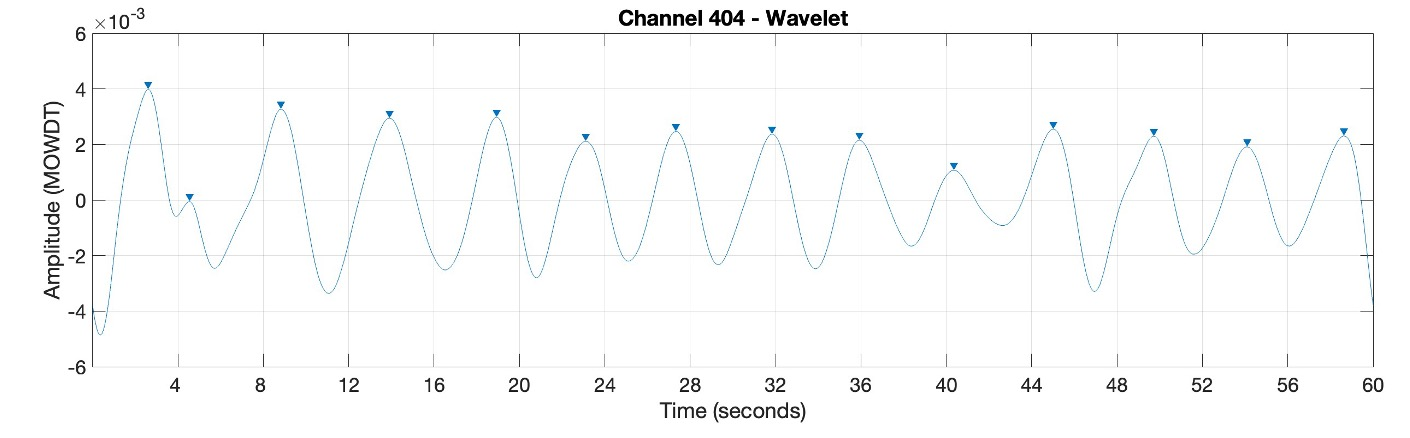
\includegraphics[width=\textwidth]{img/404_wave.jpg}
\caption{Raw data and denoised signal using MODWTMRA of the channel with the highest percentage of confidence (92\%) - Normal bed and supine position}
  \label{fig:rec}
\end{figure}

\clearpage
%%%%%% NORMAL BED - RIGHT %%%%%%
\subsubsection{Result Normal Bed in Right Side Position}   \label{cap:ResultNormalBed4}

The estimated respiratory rate per minute (rpm) while the participants are on the right side with the mattress placed on a normal bed is further presented. Table \ref{tab:RightNormalStill} presented the estimated rpm using binary and weighted approach compared with the rpm given by the ground truth. The approaches retrieve an almost identical rpm, this result may be due to the choice of the minimum confidence value at 80\% that allows keeping only the best signal, maybe with higher confidence can be seen a higher difference between the two approaches. 

\vspace{1cm}
%\begin{table}\begin{tabular}{|llllll|}
\hline 
Binary SGf & binary Waveleft & weighed  SGf & weighed Waveleft & resp rate & toolbox \\ 
\hline 
13.375 & 14.6364 & 13.375 & 14.6364 & 11.2045 & 10 \\ 
13.6667 & 15 & 13.6667 & 15 & 12.7397 & 11 \\ 
14 & 16 & 13.5 & 15.25 & 13.0613 & 12 \\ 
14.3571 & 14.2 & 14.3571 & 14.2 & 12.2669 & 12 \\ 
14 & 19 & 14 & 19 & 12.1628 & 13 \\ 
12.8 & 15 & 12.6667 & 14.5 & 13.6039 & 13 \\ 
11.8 & 14.2222 & 11.8 & 14.2222 & 13.1398 & 13 \\ 
14 & 15.6667 & 14 & 15.6667 & 11.5445 & 14 \\ 
13.8333 & 14.7 & 13.8333 & 14.7 & 10.77 & 11 \\ 
13.8889 & 15.8571 & 13.8889 & 15.8571 & 14.2216 & 12 \\ 
13.0833 & 15.5556 & 13.0833 & 15.5556 & 13.1656 & 12 \\ 
14.1111 & 16.5714 & 13.7 & 16.5714 & 12.9764 & 12 \\ 
14.2 & 15 & 14.2 & 15 & 10.9055 & 13 \\ 
13.25 & 15.125 & 13.25 & 15.125 & 13.2294 & 11 \\ 
12.7692 & 15.7143 & 12.2857 & 15.5 & 12.8524 & 11 \\ 
13.9167 & 15.2 & 13.6154 & 15.2 & 11.3824 & 13 \\ 
13 & 14.6 & 13 & 14.6 & 13.5579 & 11 \\ 
13 & 15.8889 & 13 & 15.8889 & 11.6069 & 12 \\ 
\hline 
\end{tabular}
\caption{Breath per minutes for each approach, result from Noxtural and toolbox
- Left position still mattress}
\end{table}


\begin{table}[H]
    \centering
    \begin{tabular}{|c|c|c|}
    \hline 
    Binary & Weighed  & RPM (NOXA1) \\ 
    
    \hline 
     16.1667   & 16.1667 & 12.4771 \\ 
     17.75  & 17.75 & 13.0835 \\ 
      16.5   & 16.5 & 14.3858 \\  
     15.25   & 15.25 & 12.7261 \\ 
  15.8333   & 15.8333 & 13.4867 \\ 
     15   & 15 & 12.9816 \\ 
     15.2353 &   15.2353 & 14.0566 \\ 
      15.1667  & 15.1667 & 12.038 \\ 
     15.5  & 15.5 & 11.4923 \\ 
     13  & 13 & 11.9625 \\ 
     13.3333   & 13.5 & 11.0151 \\ 
      15.5   & 15.5 & 11.9016 \\ 
     14.3333  & 14.3333 & 11.4255 \\ 
   13.8333  & 13.8333 & 12.5227 \\  
     15.2   & 15.2 & 11.5945 \\ 
      14.0909   & 14.0909 & 13.4141 \\  
     14.5   & 14.4286 & 13.5282 \\ 
      15.2308   & 15.2308 & 12.9839 \\ 
    \hline 
    \end{tabular}
    \caption{Estimated rpm using binary and weighted approach of the pipeline
    compared with the rpm given by the ground truth - Normal bed and right side}
    \label{tab:RightNormalStill}
    \end{table}

\vspace{0.5cm}

Table \ref{tab:RightNormalStillMetrics} present the average rpm for both approaches  
and the relative mean absolute error (MAE) and mean absolute percentage error (MAPE). As just discussed in the previous paragraphs there is no substantial difference between the two different approaches. The data on which to focus more is the number of breaths that the algorithm misses, represented by MAE and expressed in percentage by MAPE. The average number is 2.5rpm, which means that if we consider the estimated average of 15rpm the error is almost 20\%, worst than in the supine position but better than in the prone position and left side.

\vspace{1cm}
\begin{table}[H]
    \centering
    \begin{tabular}{|c|c|c|}
    \hline 
    & Binary  & Weighed \\ 
    \hline 
    rpm mean & 15.015 & 15.020\\
    MAE resp &  2.4638  &  2.4691  \\ 
    MAPE  &  19.9146 \%&  19.9693 \%\\ 
    \hline 
    \end{tabular}
    
    \caption{Evarage number of breath for each approach with the relative mean
    absolute error (MAE) and mean absolute percentage error (MAE) - Normal bed
    and right side}
    \label{tab:RightNormalStillMetrics}
    \end{table}
    
\vspace{0.5cm}

Figure \ref{fig:baln4} show the Bland–Altman plot, presented in section \ref{cap:plottino}, of the estimated rpm from the pipeline compared to the value of the ground truth. It helps to visualize the data from Table \ref{tab:RightNormalStillMetrics} in respect of the error. Since the result for the approaches is similar the data presented with this plot refers to the weighted approach only.

Figure \ref{fig:rec4} shows the denoised signal using MODWTMRA with the highest accuracy (92\%) for the supine position with a normal mattress.

\begin{figure}[p]
  \centering
  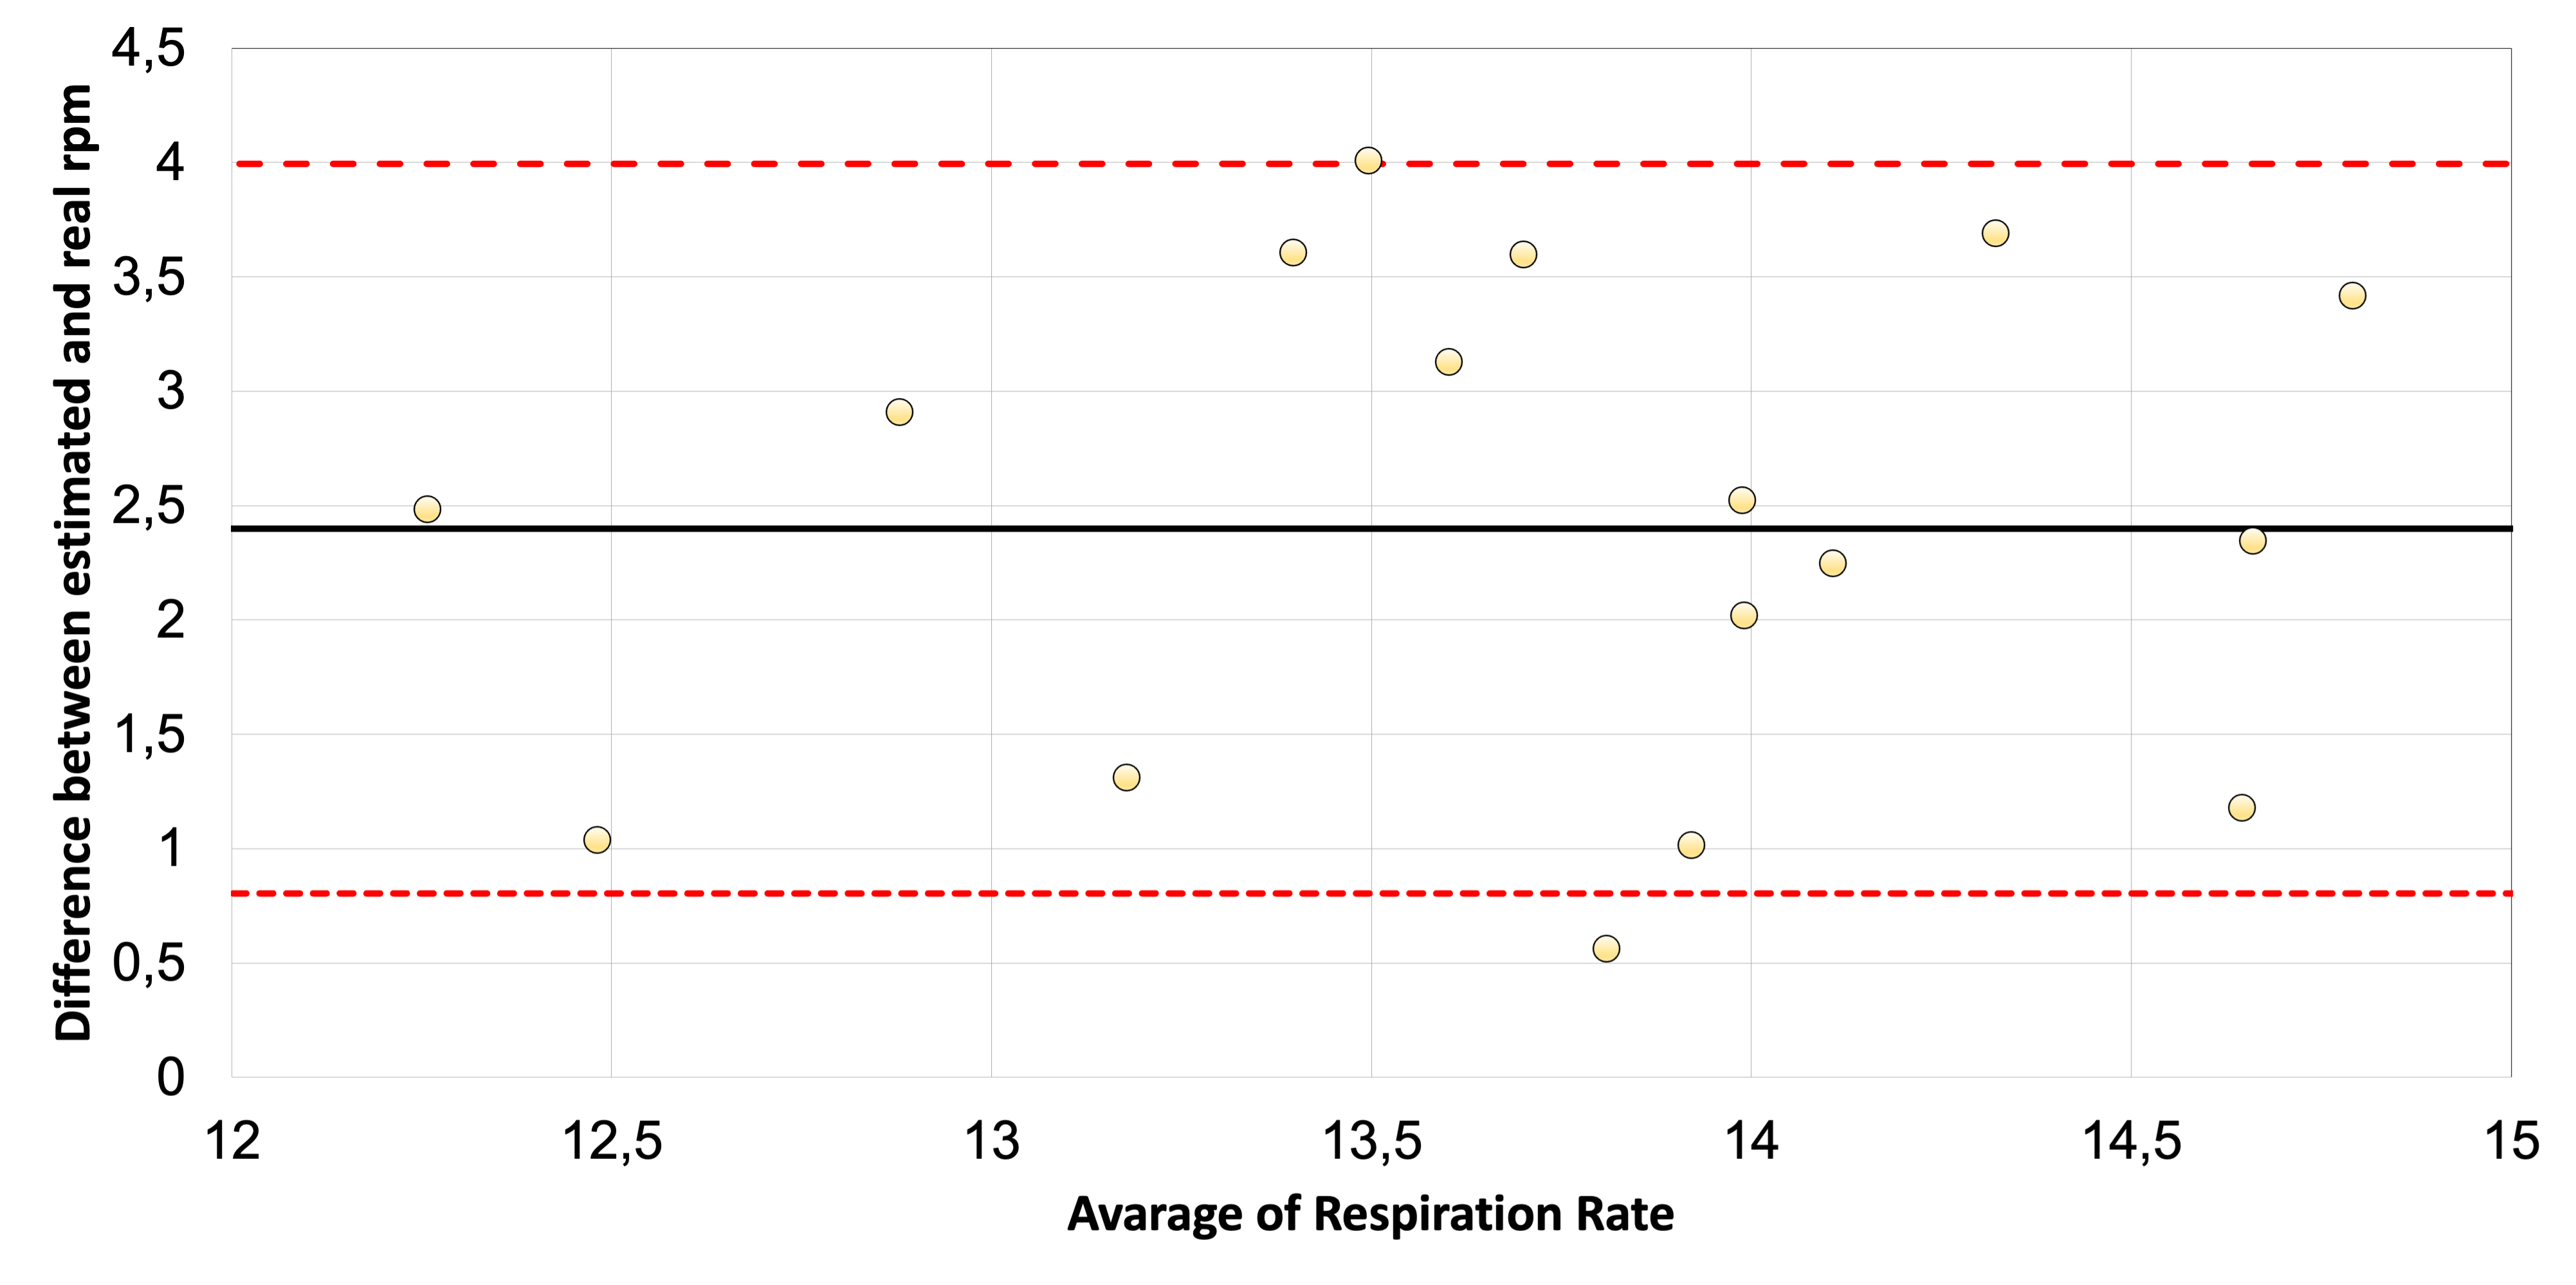
\includegraphics[width=\textwidth]{img/balnd4.png}

  \caption{Bland Altman Plot of estimated rpm from the pipeline compared to the value of the ground truth - Normal bed and left side}
  \label{fig:baln4}
  \vspace{1.5cm}
  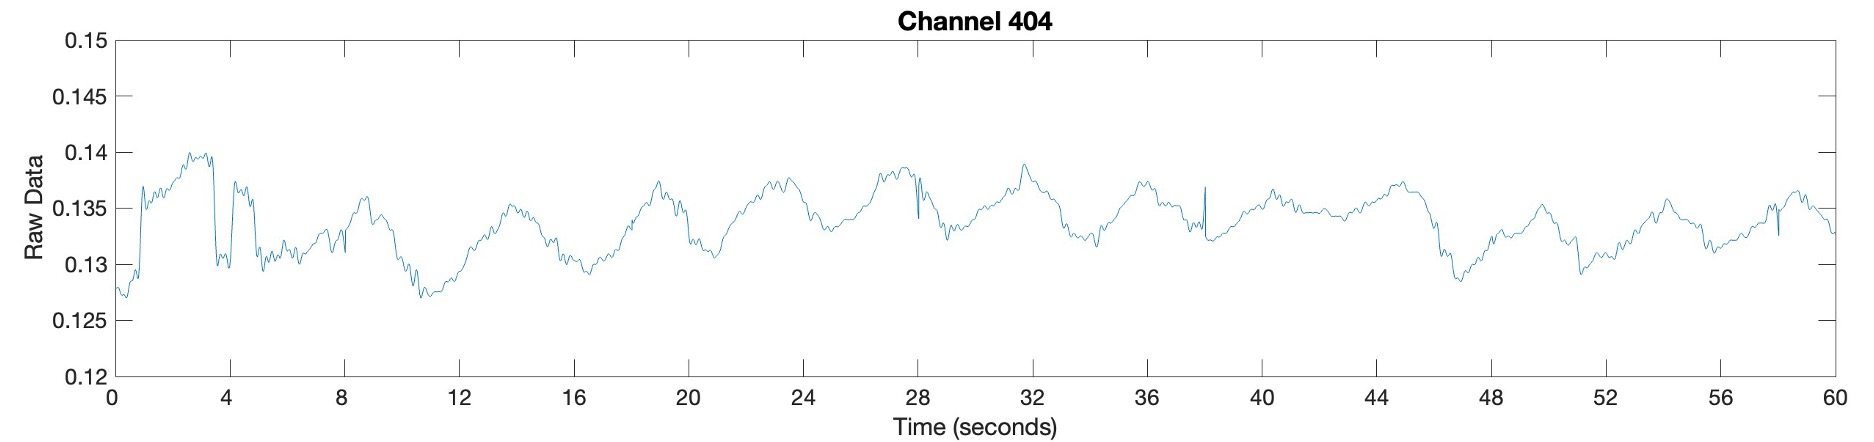
\includegraphics[width=\textwidth]{img/404.jpg}
  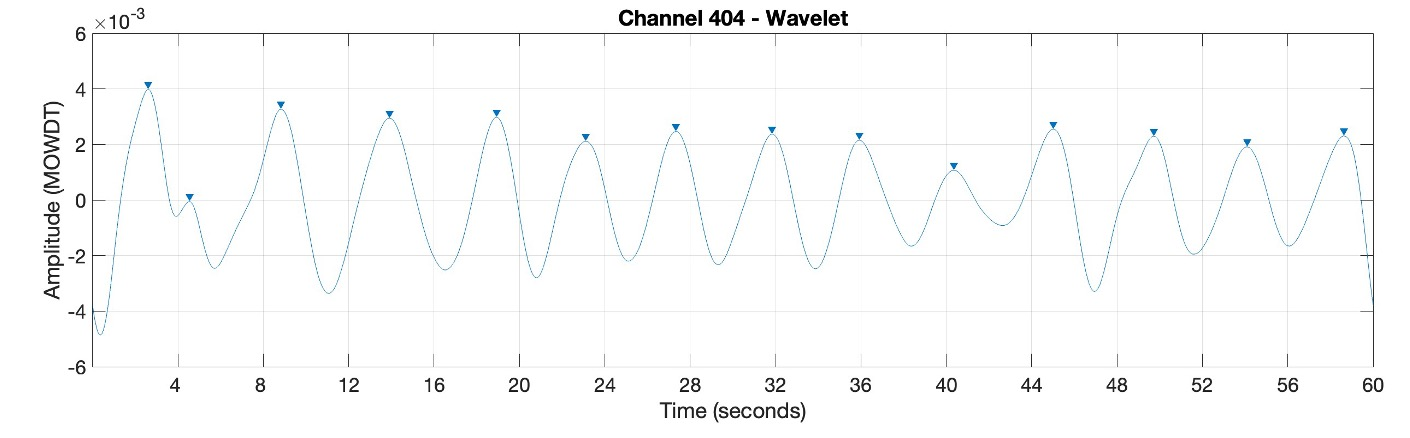
\includegraphics[width=\textwidth]{img/404_wave.jpg}
\caption{Raw data and denoised signal using MODWTMRA of the channel with the highest percentage of confidence (92\%) - Normal bed and supine position}
  \label{fig:rec4}
\end{figure}

\clearpage
%%%%%% Rocking  Bed %%%%%%
\subsection{Rocking Bed}\label{cap:RockSavitx}
The second part of the data collection aims to understand if the movement of the
rocking bed could influence the signal. The participant has to lie on the mattress without jumps, to have less variability in the data. For this phase, the mattress is placed on a rocking bed, which periods have been fixed at 4 seconds (15 periods in a minute) with an acceleration of 0.25 $m/s^2$.


%%%%%% Rocking BED - SUPINE %%%%%%

\subsubsection{Result Rocking Bed in Supine Position}  % \label{cap:ResultNormalBed1}

The estimated respiratory rate per minute (rpm) while the participants are supine with the mattress placed on a rocking bed is further presented. 

Table \ref{tab:SupineMov} presented the estimated rpm using binary and weighted approach compared with the rpm given by the ground truth. The approaches retrieve an almost identical rpm. 

\vspace{0.5cm}
\begin{table}[H]
    \centering
    \begin{tabular}{|c|c|c|}
    \hline 
    Binary & Weighed  & RPM (NOXA1) \\ 
    \hline
15.5       &  15.5    &  10.7609 \\ 
16.1333     & 16.1333  &    11.3077 \\ 
15.3333    &  15.3333   &   13.1449 \\ 
14.9474    &  14.9474    &  11.3366 \\ 
15.1       &  15.1     & 12.7314 \\ 
15.6364   &   15.6364   &   11.8892 \\ 
14.6923    &  14.6923    &    11.42 \\ 
15.2222    &  15.2222    &  13.0092 \\ 
15.1667    &  15.1667    &  13.2539 \\ 
14.6667    &  14.6667    &  11.6391 \\ 
15         &  15    &  12.2165 \\ 
14.75       & 14.75  &    11.9216 \\ 
15           &15    &  11.3091 \\ 
14.625    &   14.625   &   13.8905 \\ 
15.6154    &  15.6154   &   11.3344 \\ 
15   &   14.8182   &   11.4474 \\ 
15.1765   &   15.1765   &   11.6675 \\ 
14.6154  &    14.6154    &  13.4799 \\
\hline 
    \end{tabular}
\caption{Estimated rpm using binary and weighted approach of the pipeline compared with the rpm given by the ground truth - Rocking bed and supine position}
\label{tab:SupineMov}
\end{table}

Table \ref{tab:SupineMov} present the average rpm for both approaches  
and the relative mean absolute error (MAE) and mean absolute percentage error (MAPE). As just discussed in the previous paragraph there is no substantial difference between the two different approaches. The data on which to focus more is the number of breaths that the algorithm misses, represented by MAE and expressed in percentage by MAPE. The average number is 3rpm, which means that if we consider the estimated average of 15.1rpm the error is almost 25\%, is too high for an approach that must be used in the medical field.

%\vspace{0.5cm}

\begin{table}[h]

    \centering

\begin{tabular}{|c|c|c|c|c|}
\hline 
& Binary & Weighed \\ 
 
\hline 
rpm mean & 15.1211  & 15.1110 \\  
MAE resp   & 3.0234 &     3.0133 \\ 
MAPE resp  & 25.7324\% &  25.6442\% \\ 

\hline 
\end{tabular}
\caption{Evarage number of breath for each approach with the relative mean
absolute error (MAE) and mean absolute percentage error (MAE) - Rocking bed
and right side}
\label{tab:SupineRockingMetrics}
\end{table}

Figure \ref{fig:baln1} show the Bland–Altman plot, presented in section \ref{cap:plottino}, of the estimated rpm from the pipeline compared to the value of the ground truth. It helps to visualize the data from Table \ref{tab:SupineRockingMetrics} in respect of the error. Since the result for the approaches is similar the data presented with this plot refers to the weighted approach only.

Figure \ref{fig:rec} shows the denoised signal using MODWTMRA with the highest accuracy (92\%) for the supine position with a normal mattress.

\begin{figure}[p]
  \centering
  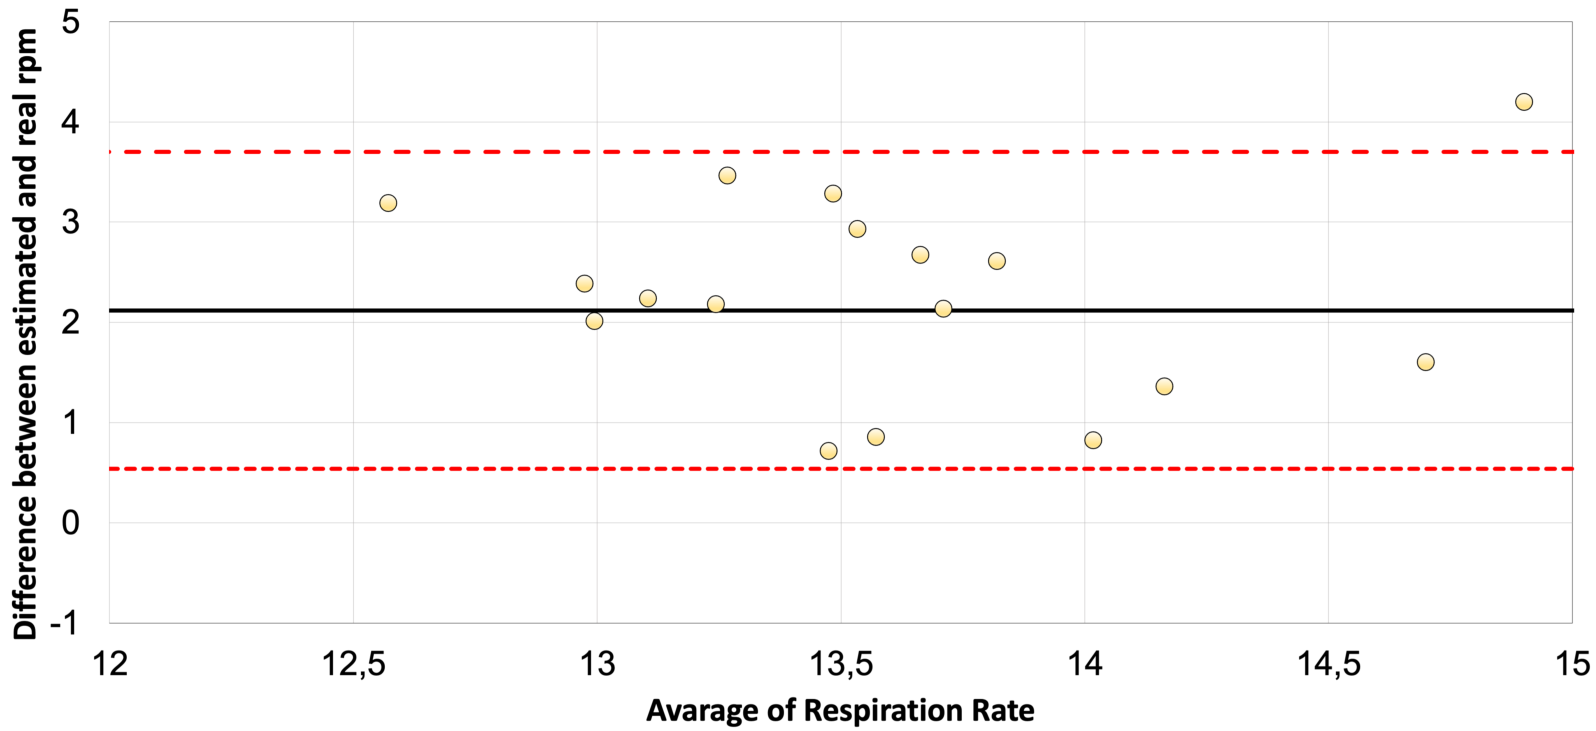
\includegraphics[width=\textwidth]{img/balnd1.pdf}

  \caption{Bland Altman Plot of estimated rpm from the pipeline compared to the value of the ground truth - Rocking bed and supine position}
  \label{fig:baln1}
  \vspace{1.5cm}
  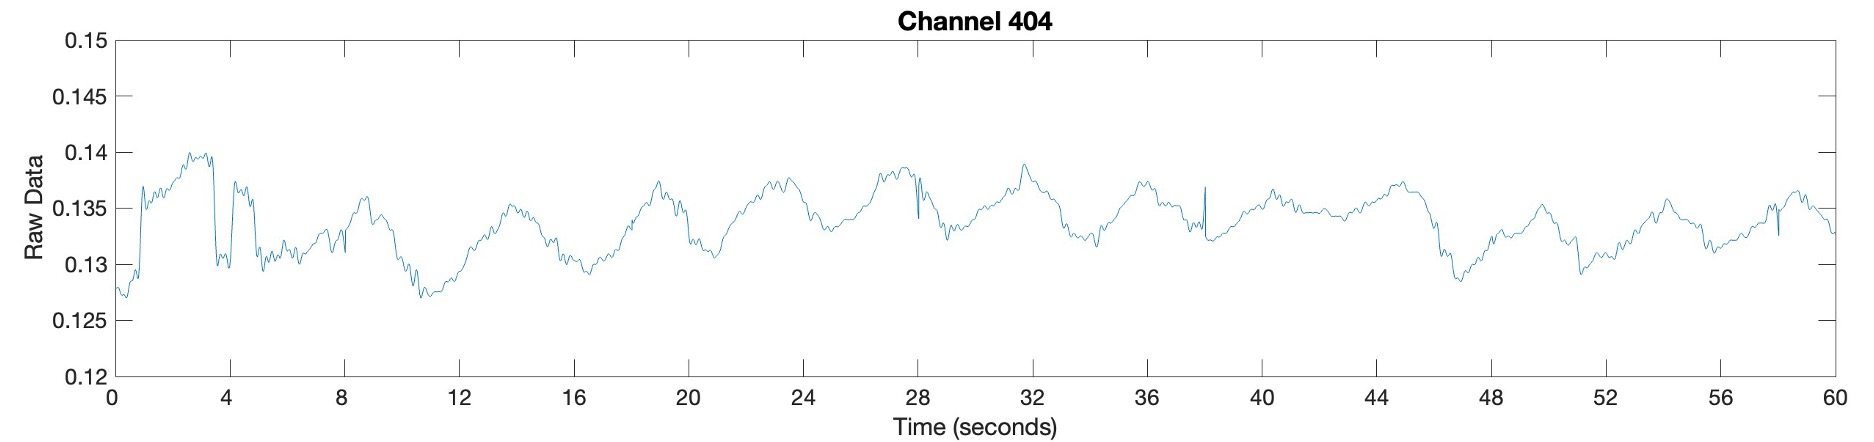
\includegraphics[width=\textwidth]{img/404.jpg}
  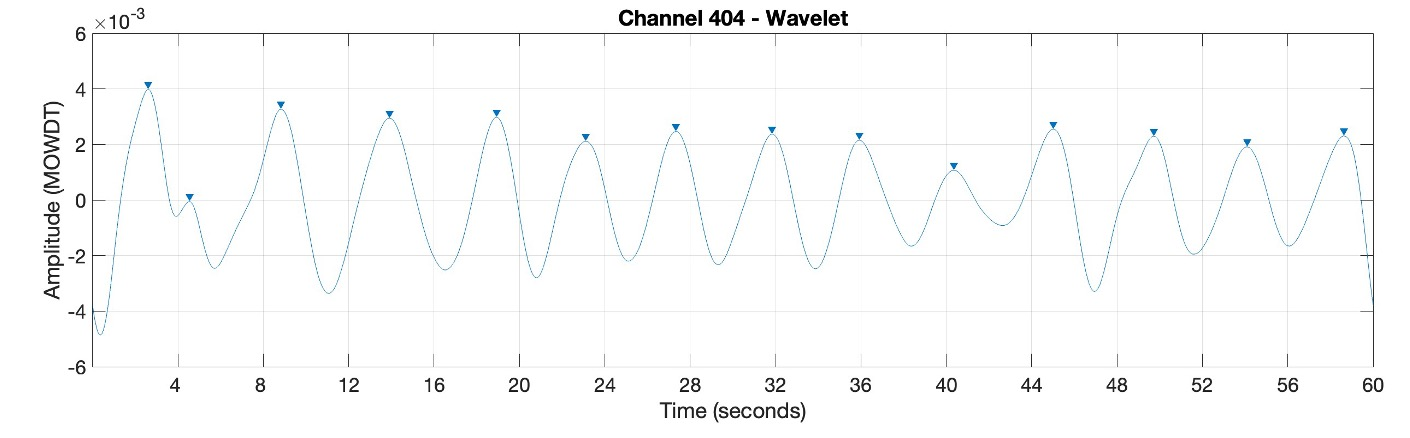
\includegraphics[width=\textwidth]{img/404_wave.jpg}
\caption{Raw data and denoised signal using MODWTMRA of the channel with the highest percentage of confidence (92\%) - Normal bed and supine position}
  \label{fig:rec}
\end{figure}

\clearpage
%%%%%% Rocking BED - LEFT %%%%%%
\subsubsection{Result Rocking Bed in Left Side Position}  % \label{cap:ResultNormalBed1}

The estimated respiratory rate per minute (rpm) while the participants are in left side position with the mattress placed on a rocking bed is further presented. 

Table \ref{tab:LeftMov} presented the estimated rpm using binary and weighted approach compared with the rpm given by the ground truth. The approaches retrieve an almost identical rpm. 

\vspace{0.5cm}
\begin{table}[H]
    \centering
    \begin{tabular}{|c|c|c|}
    \hline 
    Binary & Weighed  & RPM (NOXA1) \\ 
    \hline
15.0625   &   15.0625    &  13.6613 \\ 
15.5556   &   15.5556    &  11.4545 \\ 
15.8824    &  15.8824    &  12.3288 \\ 
16.1176   &   16.1176   &   10.8865 \\ 
15.2083    &  15.2083   &   11.4082 \\ 
15.3214    &  15.3103   &   12.2589 \\ 
15.4583   &   15.4583    &  13.7093 \\ 
15.4375   &   15.4375   &   12.7019 \\ 
15.2353    &  15.2353  &    13.3305 \\ 
15.5556   &   15.5556  &    13.7078 \\ 
15.2143    &  15.2143   &   13.5674 \\ 
15.2    &  15.1538   &   11.8694 \\ 
15.5556    &  15.5556   &   13.4086 \\ 
14.75      &  14.75   &   13.9781 \\ 
14.5      &   14.5   &   12.4749 \\ 
15.25     &   15.25   &   12.4049 \\ 
14.625    &  14.7273   &   13.4108 \\ 
14.2857   &   14.3333   &   13.4716 \\ 
\hline 
    \end{tabular}
\caption{Estimated rpm using binary and weighted approach of the pipeline compared with the rpm given by the ground truth - Rocking bed and left side}
\label{tab:LeftMov}
\end{table}

Table \ref{tab:LeftMov} present the average rpm for both approaches  
and the relative mean absolute error (MAE) and mean absolute percentage error (MAPE). As just discussed in the previous paragraph there is no substantial difference between the two different approaches. The data on which to focus more is the number of breaths that the algorithm misses, represented by MAE and expressed in percentage by MAPE. The average number is 2.5rpm, which means that if we consider the estimated average of 15.2rpm the error is almost 20\%, which is too high for an approach that must be used in the medical field.

%\vspace{0.5cm}
\begin{table}[h]
    \centering
    \begin{tabular}{|c|c|c|}
    \hline 
    & Binary & Weighed \\ 
    
    \hline 
    rpm mean & 15.2342  & 15.2393  \\
    MAE resp  &   2.4545 &  2.4597 \\ 
    MAPE resp  & 19.9605 \% & 19.9959 \%\\ 
    \hline 
\end{tabular}
\caption{Evarage number of breath for each approach with the relative mean
absolute error (MAE) and mean absolute percentage error (MAE) - Rocking bed
and left side}
\label{tab:LeftRockingMetrics}
\end{table}

Figure \ref{fig:baln1} show the Bland–Altman plot, presented in section \ref{cap:plottino}, of the estimated rpm from the pipeline compared to the value of the ground truth. It helps to visualize the data from Table \ref{tab:LeftRockingMetrics} in respect of the error. Since the result for the approaches is similar the data presented with this plot refers to the weighted approach only.

Figure \ref{fig:rec} shows the denoised signal using MODWTMRA with the highest accuracy (92\%) for the supine position with a normal mattress.

\begin{figure}[p]
  \centering
  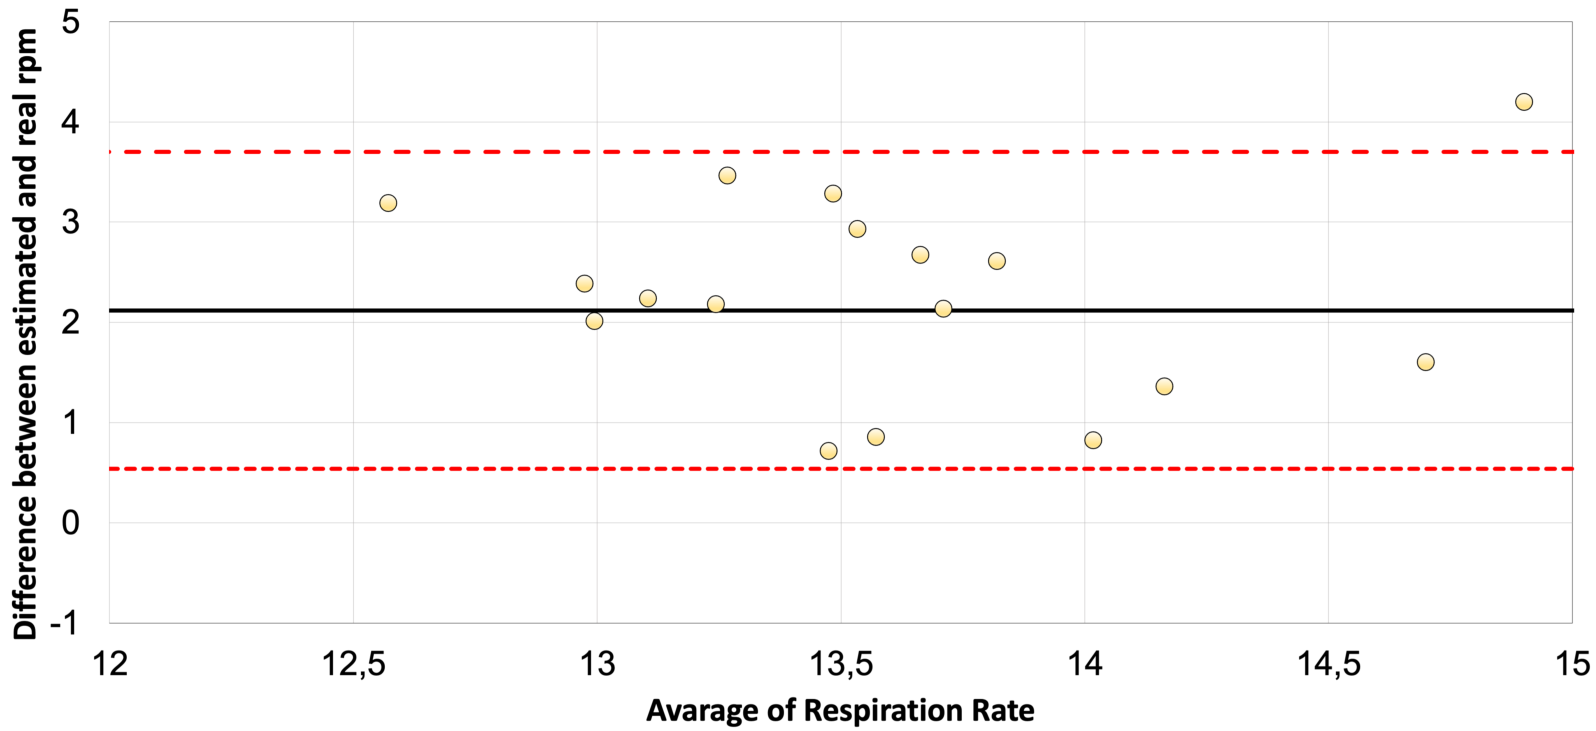
\includegraphics[width=\textwidth]{img/balnd1.pdf}

  \caption{Bland Altman Plot of estimated rpm from the pipeline compared to the value of the ground truth - Normal bed and supine position}
  \label{fig:baln1}
  \vspace{1.5cm}
  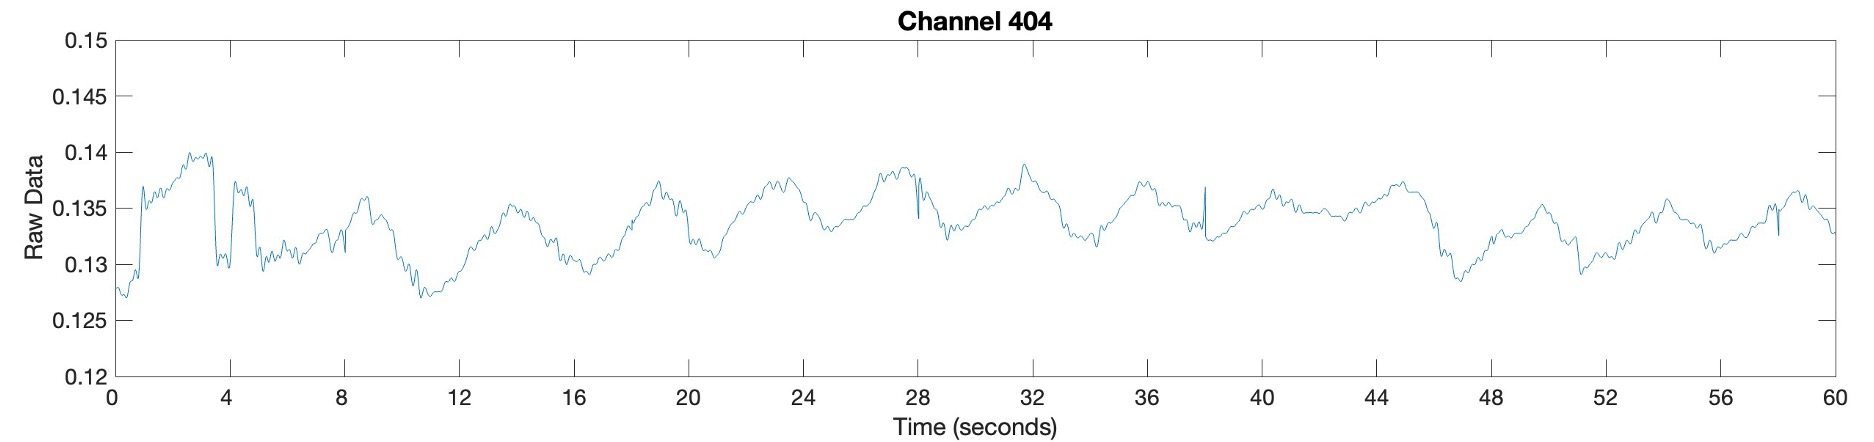
\includegraphics[width=\textwidth]{img/404.jpg}
  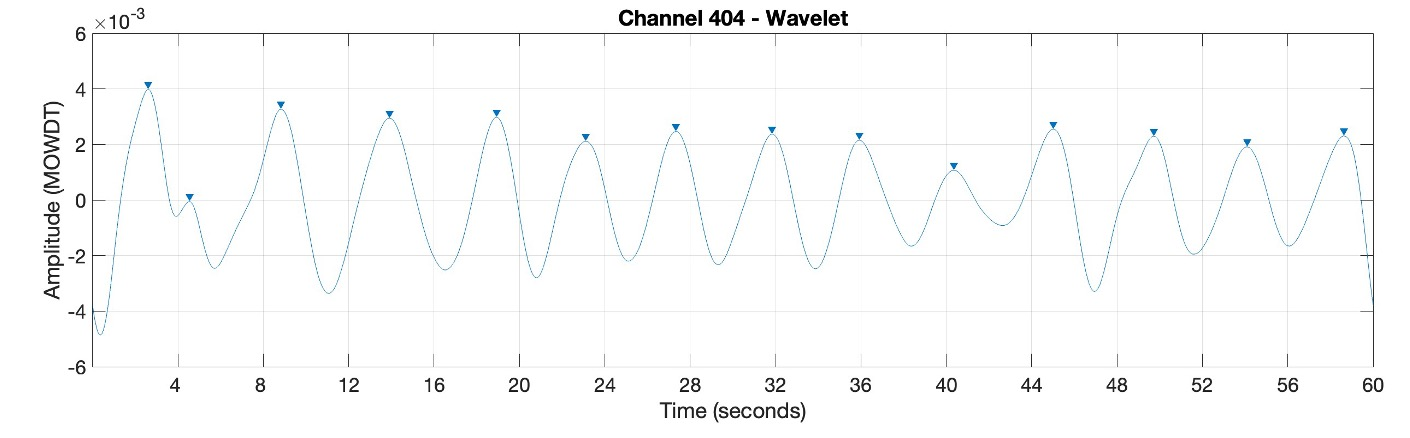
\includegraphics[width=\textwidth]{img/404_wave.jpg}
\caption{Raw data and denoised signal using MODWTMRA of the channel with the highest percentage of confidence (92\%) - Normal bed and supine position}
  \label{fig:rec}
\end{figure}

\clearpage
%%%%%% Rocking BED - Prone %%%%%%
\subsubsection{Result Rocking Bed in Prone Position}  % \label{cap:ResultNormalBed1}

The estimated respiratory rate per minute (rpm) while the participants are in prone position with the mattress placed on a rocking bed is further presented. 

Table \ref{tab:LeftMov} presented the estimated rpm using binary and weighted approach compared with the rpm given by the ground truth. The approaches retrieve an almost identical rpm. 

\vspace{0.5cm}
\begin{table}[h]
    \centering
    \begin{tabular}{|c|c|c|}
 
    \hline 
    Binary & Weighed &RPM (NOXA1) \\ 
    \hline 
16         &    16     &   12.6296 \\ 
15.3684     &   15.3684    &     14.168 \\ 
15.6818    &    15.6818   &     13.2588 \\ 
15.5     &   15.4286    &    13.8107 \\ 
15.8333    &    15.8333    &     13.485 \\ 
16        &     16   &     12.6052 \\ 
16        &     16   &     11.0417 \\ 
15.7059    &    15.7059   &     12.9088 \\ 
15.5333    &    15.5333   &     13.0502 \\ 
16.3333    &    16.3333  &      11.1723 \\ 
14.5625     &   14.5625   &     14.6869 \\ 
15.5294    &    15.5294   &     11.3484 \\ 
14.7273    &    14.7273   &     13.0399 \\ 
14.7778    &    14.7778   &     9.54872 \\ 
15.4444     &   15.4444   &     11.7918 \\ 
14.9286    &    14.9286   &     12.8182 \\ 
15.8333    &    15.8333   &     9.53453 \\ 
14.619     &    14.619    &     9.5416 \\ 
\hline 
\end{tabular}
\caption{Estimated rpm using binary and weighted approach of the pipeline
compared with the rpm given by the ground truth
- Rocking bed and prone position}
\label{tab:ProneMov}

\end{table}


Table \ref{tab:ProneRockingMetrics} present the average rpm for both approaches  
and the relative mean absolute error (MAE) and mean absolute percentage error (MAPE). As just discussed in the previous paragraph there is no substantial difference between the two different approaches. The data on which to focus more is the number of breaths that the algorithm misses, represented by MAE and expressed in percentage by MAPE. The average number is 2.5rpm, which means that if we consider the estimated average of 15.2rpm the error is almost 20\%, which is too high for an approach that must be used in the medical field.

%\vspace{0.5cm}
\begin{table}[h]
    \centering
    \begin{tabular}{|c|c|c|}
    \hline 
    & Binary & Weighed \\ 
    
    \hline 
    rpm mean & 15.4655  & 15.4615  \\
MAE resp   &   3.2326   &  3.2286 \\ 
MAPE resp   & 28.5509   & 28.5221 \\ 
    \hline 
\end{tabular}
\caption{Evarage number of breath for each approach with the relative mean
absolute error (MAE) and mean absolute percentage error (MAE) - Rocking bed
and prone position}
\label{tab:ProneRockingMetrics}
\end{table}

Figure \ref{fig:baln1} show the Bland–Altman plot, presented in section \ref{cap:plottino}, of the estimated rpm from the pipeline compared to the value of the ground truth. It helps to visualize the data from Table \ref{tab:ProneRockingMetrics} in respect of the error. Since the result for the approaches is similar the data presented with this plot refers to the weighted approach only.

Figure \ref{fig:rec} shows the denoised signal using MODWTMRA with the highest accuracy (92\%) for the supine position with a normal mattress.

\begin{figure}[p]
  \centering
  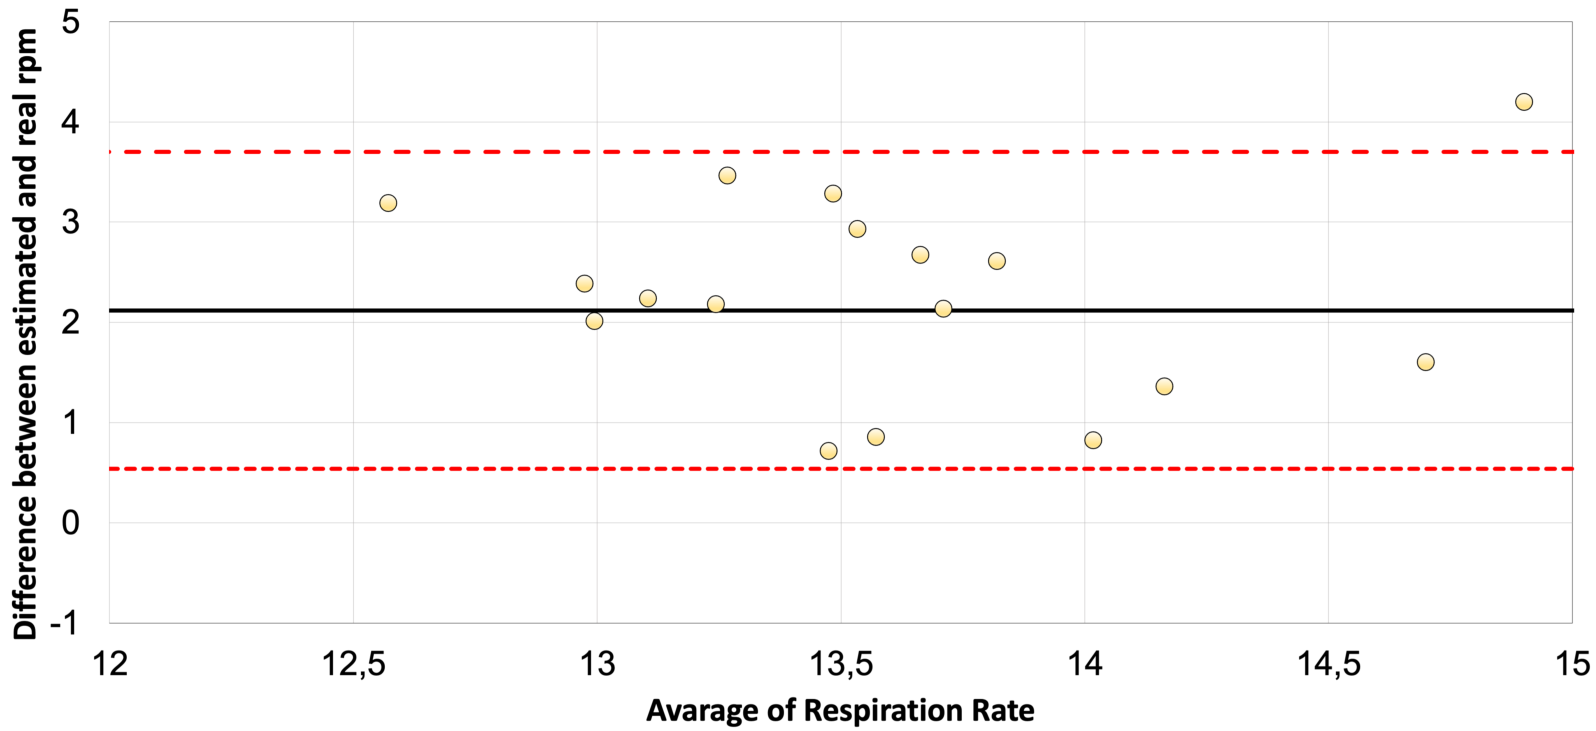
\includegraphics[width=\textwidth]{img/balnd1.pdf}

  \caption{Bland Altman Plot of estimated rpm from the pipeline compared to the value of the ground truth - Normal bed and supine position}
  \label{fig:baln1}
  \vspace{1.5cm}
  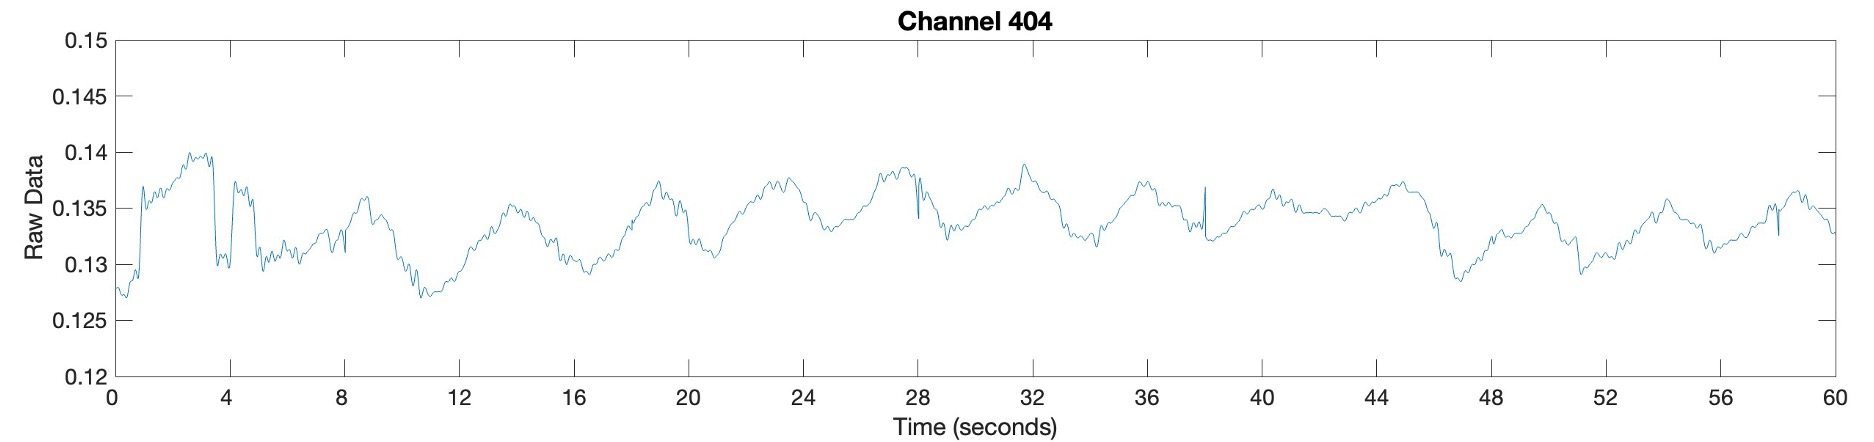
\includegraphics[width=\textwidth]{img/404.jpg}
  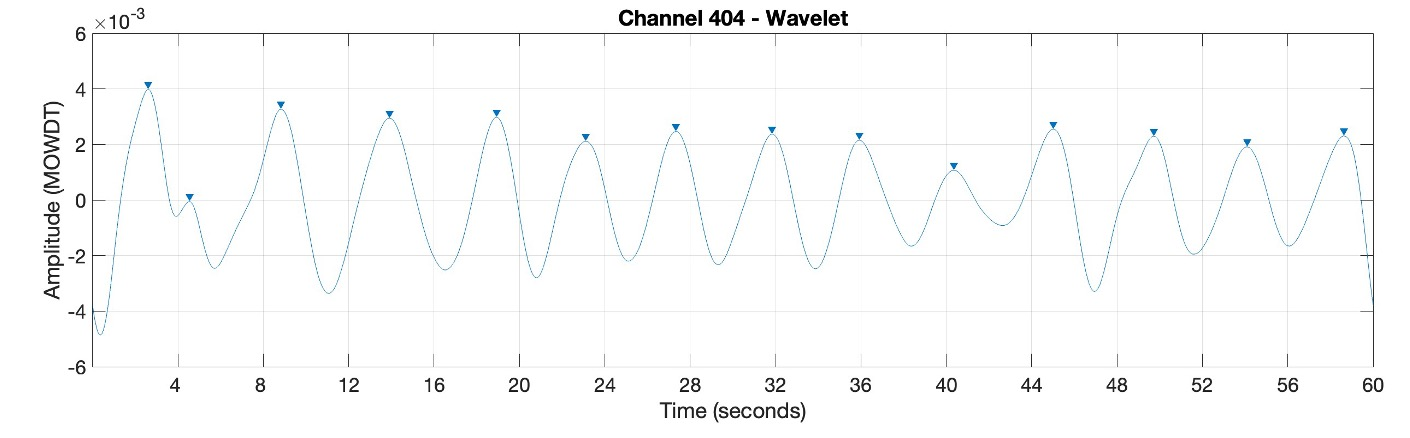
\includegraphics[width=\textwidth]{img/404_wave.jpg}
\caption{Raw data and denoised signal using MODWTMRA of the channel with the highest percentage of confidence (92\%) - Normal bed and supine position}
  \label{fig:rec}
\end{figure}

\clearpage
%%%%%% Rocking BED - RIGHT %%%%%%
\subsubsection{Result Rocking Bed in Right Side }  % \label{cap:ResultNormalBed1}

The estimated respiratory rate per minute (rpm) while the participants are in right side position with the mattress placed on a rocking bed is further presented. 

Table \ref{tab:RightMov} presented the estimated rpm using binary and weighted approach compared with the rpm given by the ground truth. The approaches retrieve an almost identical rpm. 

\vspace{0.5cm}
\begin{table}[h]
    \centering
    \begin{tabular}{|c|c|c|}
 
    \hline 
    Binary & Weighed &RPM (NOXA1) \\ 
    \hline 
15.8095    &  15.8095   &   11.7955 \\ 
15.2105    &     15.1  &    11.9185 \\ 
15.5652    &  15.5652 &     11.8639 \\ 
15.8261    &  15.8261    &    12.28 \\ 
15.6667    &  15.6667   &  12.0136 \\ 
15.1176   &   15.1176   &   12.8838 \\ 
15.3571   &   15.3571  &    11.5695 \\ 
15    &  14.8696   &   12.8922 \\ 
15.1176  &    15.1176  &     11.587 \\ 
15.2857   &   15.2857  &    11.2449 \\ 
15.3333   &   15.3333   &   11.7082 \\ 
15.3684    &    15.35   &   13.9497 \\ 
15.6154    &  15.4286   &   11.6145 \\ 
15.4286    &  15.4286  &    13.9913 \\ 
15.2727    &  15.2727   &   11.6172 \\ 
15.3      &  15.3    &  13.3257 \\ 
15.1667   &   15.1667  &    13.5179 \\ 
14.9231   &   14.9286   &   13.5767 \\ 
\hline 
\end{tabular}
\caption{Estimated rpm using binary and weighted approach of the pipeline
compared with the rpm given by the ground truth - Rocking bed and right side position}
\label{tab:RightMov}

\end{table}

Table \ref{tab:RightMov} present the average rpm for both approaches  
and the relative mean absolute error (MAE) and mean absolute percentage error (MAPE). As just discussed in the previous paragraph there is no substantial difference between the two different approaches. The data on which to focus more is the number of breaths that the algorithm misses, represented by MAE and expressed in percentage by MAPE. The average number is 2.9rpm, which means that if we consider the estimated average of 15.3rpm the error is almost 24\%, which is too high for an approach that must be used in the medical field.

%\vspace{0.5cm}

\begin{table}
    \centering 
    \begin{tabular}{|c|c|c|}
    \hline 
    & Binary & Weighed  \\ 
    
    \hline 
    rpm mean &15.3536  & 15.3291 \\
    MAE resp & 2.9452 &      2.9208 \\ 
    MAPE  & 24.4008 \%& 24.1986\% \\ 
    \hline 
\end{tabular}
\caption{Evarage number of breath for each approach with the relative mean
absolute error (MAE) and mean absolute percentage error (MAE) - Rocking bed
and right side}
\label{tab:RightRockingMetrics}
\end{table}

Figure \ref{fig:baln1} show the Bland–Altman plot, presented in section \ref{cap:plottino}, of the estimated rpm from the pipeline compared to the value of the ground truth. It helps to visualize the data from Table \ref{tab:RightRockingMetrics} in respect of the error. Since the result for the approaches is similar the data presented with this plot refers to the weighted approach only.

Figure \ref{fig:rec} shows the denoised signal using MODWTMRA with the highest accuracy (92\%) for the supine position with a normal mattress.

\begin{figure}[p]
  \centering
  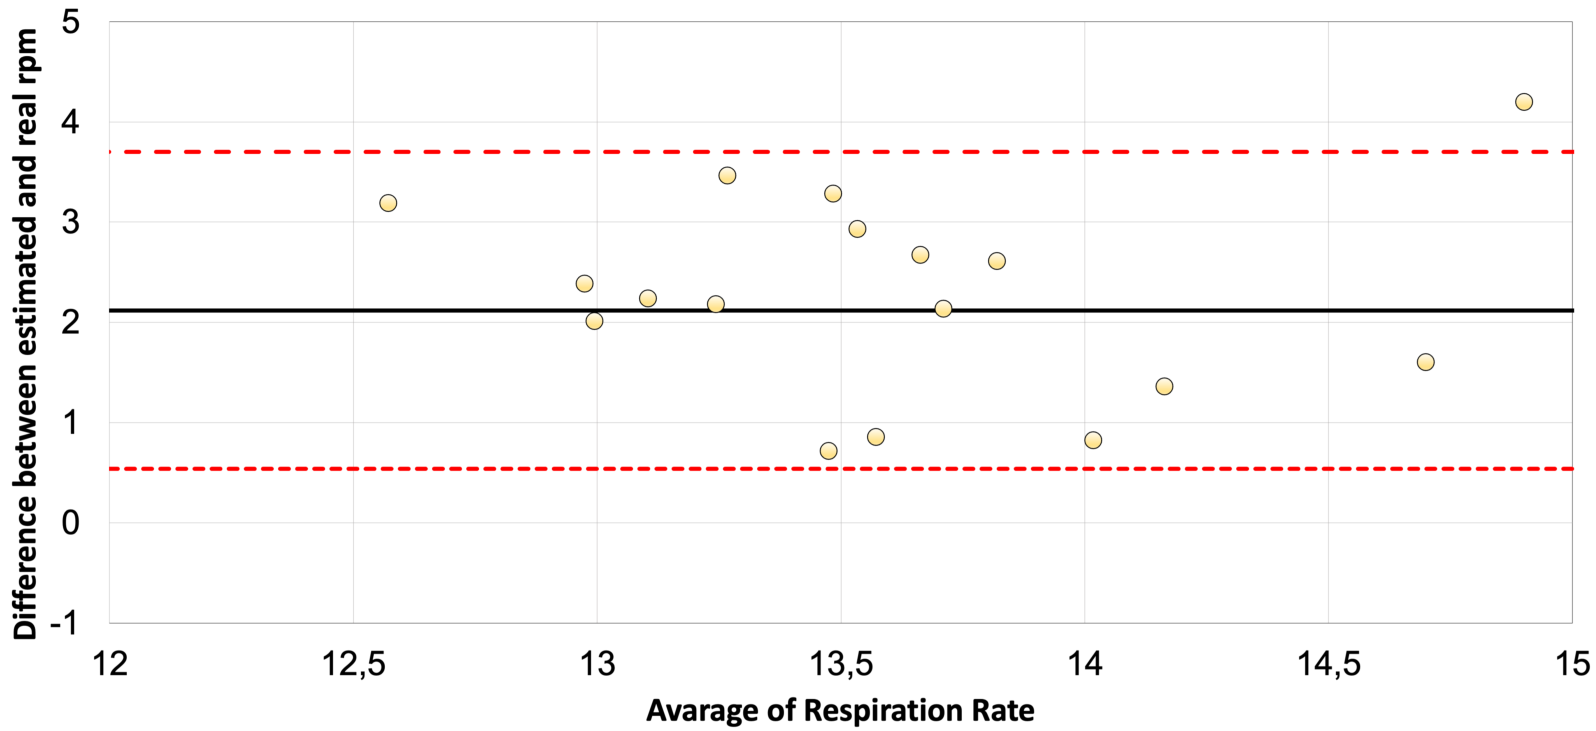
\includegraphics[width=\textwidth]{img/balnd1.pdf}

  \caption{Bland Altman Plot of estimated rpm from the pipeline compared to the value of the ground truth - Normal bed and supine position}
  \label{fig:baln1}
  \vspace{1.5cm}
  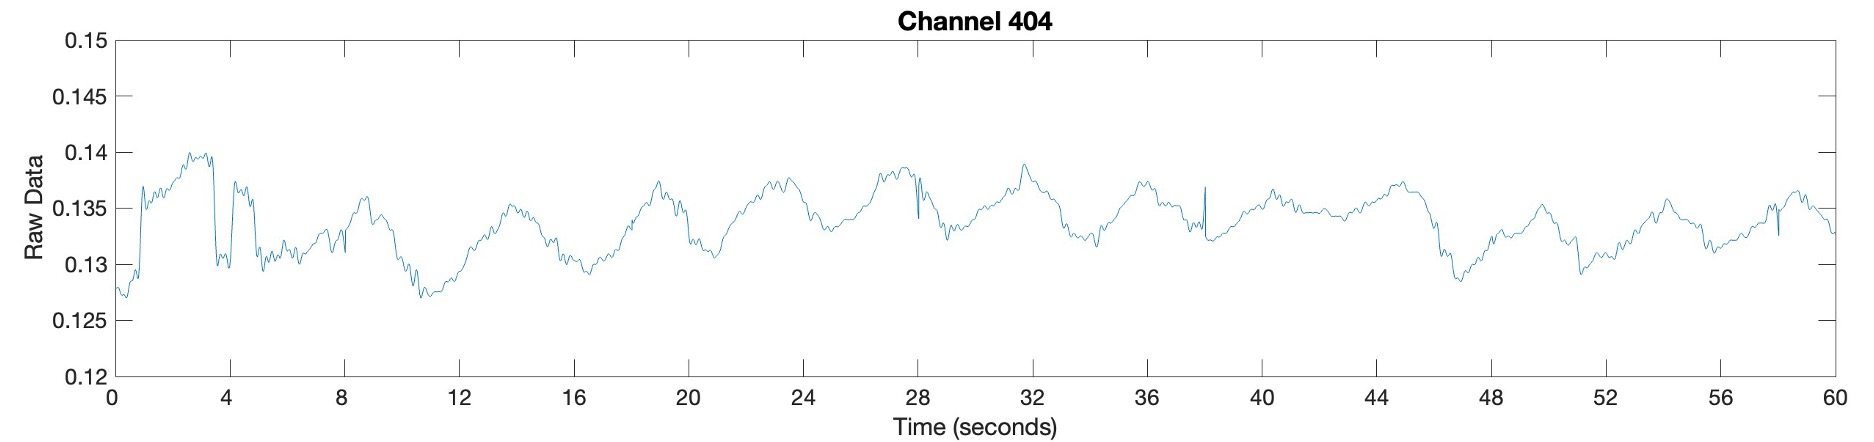
\includegraphics[width=\textwidth]{img/404.jpg}
  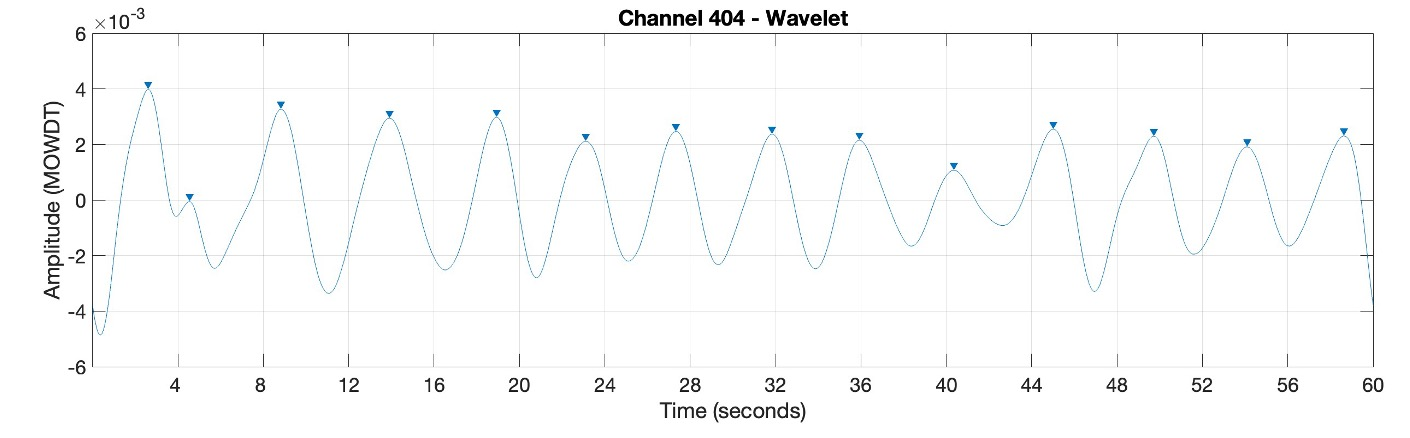
\includegraphics[width=\textwidth]{img/404_wave.jpg}
\caption{Raw data and denoised signal using MODWTMRA of the channel with the highest percentage of confidence (92\%) - Normal bed and supine position}
  \label{fig:rec}
\end{figure}